\documentclass[a4paper,11pt,twoside]{report}
\let\oldemph\emph
\renewcommand\emph[1]{{\huge{#1}}}
% THIS FILE SHOULD BE COMPILED BY pdfLaTeX

% ----------------------   PREAMBLE PART ------------------------------


% ------------------------ ENCODING & LANGUAGES ----------------------

\usepackage[utf8]{inputenc}
%\usepackage[MeX]{polski} % Not needed unless You have a name with polish symbols or sth
\usepackage[T1]{fontenc}
\usepackage[english, polish]{babel}
\usepackage{longtable}
\usepackage[section]{placeins}

\usepackage{ltablex}
\usepackage{amsmath, amsfonts, amsthm, latexsym} % MOSTLY MATHEMATICAL SYMBOLS

\usepackage[final]{pdfpages} % INPUTING TITLE PDF PAGE - GENERATE IT FIRST!
%\usepackage[backend=bibtex, style=verbose-trad2]{biblatex}

% ---------------- MARGINS, INDENTATION, LINESPREAD ------------------

\usepackage[inner=20mm, outer=20mm, bindingoffset=10mm, top=25mm, bottom=25mm]{geometry} % MARGINS


\linespread{1.5}
\allowdisplaybreaks         % ALLOWS BREAKING PAGE IN MATH MODE

\usepackage{indentfirst}    % IT MAKES THE FIRST PARAGRAPH INDENTED; NOT NEEDED
\setlength{\parindent}{5mm} % WIDTH OF AN INDENTATION


%---------------- RUNNING HEAD - CHAPTER NAMES, PAGE NUMBERS ETC. -------------------

\usepackage{fancyhdr}
\pagestyle{fancy}
\fancyhf{}
% PAGINATION: LEFT ALIGNMENT ON EVEN PAGES, RIGHT ALIGNMENT ON ODD PAGES 
\fancyfoot[LE,RO]{\thepage} 
% RIGHT HEADER: zawartość \rightmark do lewego, wewnętrznego (marginesu) 
\fancyhead[LO]{\sc \nouppercase{\rightmark}}
% lewa pagina: zawartość \leftmark do prawego, wewnętrznego (marginesu) 
\fancyhead[RE]{\sc \leftmark}

\renewcommand{\chaptermark}[1]{\markboth{\thechapter.\ #1}{}}

% HEAD RULE - IT'S A LINE WHICH SEPARATES HEADER AND FOOTER FROM CONTENT
\renewcommand{\headrulewidth}{0 pt} % 0 MEANS NO RULE, 0.5 MEANS FINE RULE, THE BIGGER VALUE THE THICKER RULE


\fancypagestyle{plain}{
  \fancyhf{}
  \fancyfoot[LE,RO]{\thepage}
  
  \renewcommand{\headrulewidth}{0pt}
  \renewcommand{\footrulewidth}{0.0pt}
}



% --------------------------- CHAPTER HEADERS ---------------------

\usepackage{titlesec}
\titleformat{\chapter}
  {\normalfont\Large \bfseries}
  {\thechapter.}{1ex}{\Large}

\titleformat{\section}
  {\normalfont\large\bfseries}
  {\thesection.}{1ex}{}
\titlespacing{\section}{0pt}{30pt}{20pt} 

    
\titleformat{\subsection}
  {\normalfont \bfseries}
  {\thesubsection.}{1ex}{}


% ----------------------- TABLE OF CONTENTS SETUP ---------------------------
\usepackage[skip=0.5\baselineskip]{caption}

\def\cleardoublepage{\clearpage\if@twoside
\ifodd\c@page\else\hbox{}\thispagestyle{empty}\newpage
\if@twocolumn\hbox{}\newpage\fi\fi\fi}
                                                                                                                                                                                                                                                                                           

% THIS MAKES DOTS IN TOC FOR CHAPTERS
\usepackage{etoolbox}
\makeatletter
\patchcmd{\l@chapter}
  {\hfil}
  {\leaders\hbox{\normalfont$\m@th\mkern \@dotsep mu\hbox{.}\mkern \@dotsep mu$}\hfill}
  {}{}
\makeatother

\usepackage{titletoc}
\makeatletter
\titlecontents{chapter}% <section-type>
  [0pt]% <left>
  {}% <above-code>
  {\bfseries \thecontentslabel.\quad}% <numbered-entry-format>
  {\bfseries}% <numberless-entry-format>
  {\bfseries\leaders\hbox{\normalfont$\m@th\mkern \@dotsep mu\hbox{.}\mkern \@dotsep mu$}\hfill\contentspage}% <filler-page-format>

\titlecontents{section}
  [1em]
  {}
  {\thecontentslabel.\quad}
  {}
  {\leaders\hbox{\normalfont$\m@th\mkern \@dotsep mu\hbox{.}\mkern \@dotsep mu$}\hfill\contentspage}

\titlecontents{subsection}
  [2em]
  {}
  {\thecontentslabel.\quad}
  {}
  {\leaders\hbox{\normalfont$\m@th\mkern \@dotsep mu\hbox{.}\mkern \@dotsep mu$}\hfill\contentspage}
\makeatother



% ---------------------- TABLES AD FIGURES NUMBERING ----------------------

\renewcommand*{\thetable}{\arabic{chapter}.\arabic{table}}
\renewcommand*{\thefigure}{\arabic{chapter}.\arabic{figure}}


% ------------- DEFINING ENVIRONMENTS FOR THEOREMS, DEFINITIONS ETC. ---------------

\makeatletter
\newtheoremstyle{definition}
{3ex}%                           % Space above
{3ex}%                           % Space below
{\upshape}%                      % Body font
{}%                              % Indent amount
{\bfseries}%                     % Theorem head font
{.}%                             % Punctuation after theorem head
{.5em}%                          % Space after theorem head, ' ', or \newline
{\thmname{#1}\thmnumber{ #2}\thmnote{ (#3)}}
\makeatother

\theoremstyle{definition}
\newtheorem{theorem}{Theorem}[chapter]
\newtheorem{lemma}[theorem]{Lemma}
\newtheorem{example}[theorem]{Example}
\newtheorem{proposition}[theorem]{Proposition}
\newtheorem{corollary}[theorem]{Corollary}
\newtheorem{definition}[theorem]{Definition}
\newtheorem{remark}[theorem]{Remark}

% --------------------- END OF PREAMBLE PART (MOSTLY) --------------------------





% -------------------------- USER SETTINGS ---------------------------

\newcommand{\tytul}{System zarządzania zasobami małego laboratorium chemicznego}
\renewcommand{\title}{A System for Resources Management in a Small Chemistry Laboratory}
\newcommand{\type}{Engineer} % Master OR Engineer
\newcommand{\supervisor}{dr inż. Agnieszka Jastrzębska} % TITLE AND NAME OF THE SUPERVISOR



\begin{document}
\sloppy
\selectlanguage{english}


\includepdf[pages=-]{titlepage} % THIS INPUTS THE TITLE PAGE


% ------------------ PAGE WITH SIGNATURES --------------------------------

\thispagestyle{empty}\newpage
\null

\vfill

\begin{center}
\begin{tabular}[t]{ccc}
............................................. & \hspace*{100pt} & .............................................\\
supervisor's signature & \hspace*{100pt} & author's signature
\end{tabular}
\end{center}



% ---------------------------- ABSTRACTS -----------------------------

{
\begin{abstract}

\begin{center}
\emph{\title}
\end{center}


Computer software is widely used amongst many areas and has become an essential part of many modern working environments. The application software serves as a replacement of traditional method of storing and accessing data and has improved those to the great extent.
The topic of this engineering thesis is a resolution of a problem of management of supplies in a small chemistry laboratory by the means of designing a implementing a dedicated computer software.  Resulting from that is a system supporting management of resources (chemical reagents, instruments, etc.). The system keeps track of the state of resources in the laboratory, and stores the data in a database. The application has graphical user-friendly interface which facilitates displaying and modifying the gathered data. Multiple functionalities in the system allow the user to classify the resource into groups and assign descriptions with multimedia content to them. What is more, the application allows the user to define and generate reports and notifications. reports are displaying current state of resources as well as plot of activity in time, plot of demand for some resource in time, bar chart, pie chart, whereas notifications are alerts about low level of some chemical reagent, etc. The system also stores suppliers’ contact data for each resource and allows the user to order new resources directly from the application. Other functionalities include the prediction of the future demand for resources based on available historical data
The implemented system is a Web Application. It consists of a client application – developed in AngularJS – and server – developed in SpringBoot Java. Elements of application exchange information using RESTful API. As for development tools, the IntelliJ IDEA (a Java integrated development environment (IDE)) was used to implement the solution.
\\

\noindent \textbf{Keywords:} Resource Management, Database, Time Series Forecast, Web Application, Java, AngularJS, SpringBoot, RESTful API, IntelliJ IDEA
\end{abstract}
}

\null\thispagestyle{empty}\newpage


{\selectlanguage{polish}
\begin{abstract}

\begin{center}
\emph{\tytul}
\end{center}

 Opragramowanie komputerowe jest obecnie używane w wielu dziedzinach życia i na codzień ułatwie pracę wielu przedsiębiorstwom. Stosowanie programów komputerowych do przechowywania i odczytywania danych, znacznie usprawniło tę dziedzinę. Przedmiotem tej pracy inżynierskiej jest aplikacja, która rozwiązała problem zarządzania zasobami małego laboratorium chemicznego, poprzez zaprojektowanie i stworzenie oprogramowania komputerowego. Wynikiem pracy stała się aplikacja, która wspomoga zarządzanie zasobami w tej instytucji (reagentami chemicznymi, sprzętem laboratoryjnym i tym podobnych). Program zbiera informacje o stanie zasobów i przechowuje je w bazie danych. Aplikacja posada przyjazny dla użytkownika interfejs graficzny, co ułatwia wy\'swietlanie i modyfikacje zebranych danych. Pozostałe funkcjonalno\'sci systemu pozwalają na przypisane zasobom opisów i multimediów (np. zdjęć) oraz ich klasyfikację w grupy. Możliwe jest również definiowanie i generowanie raportów i notyfikacji. Raporty przedstawiają obecny stan zasobów, jak również wykresy aktywno\'s ci (produkcji) albo zapotrzebowania na zasoby w czasie. Są to wykresy słupkowe, wykresy kołowe lub inne. Notyfikacje to alerty o niskim poziomie zasobów. Dla każdego zasobu, przechowaywane są informacje o danych kontaktowych do dostawcy oraz umożliwione jest zamówienie nowych bezporednio z aplikacji. Dodatkową funkcjonalno\'scię jest również przwewidywanie przyszłego zapotrzebowania na zasoby na podstawie danych historycznych. Zaimplementowany system jest aplikacją internetową. Składa się z aplikacji klienta - zaimplementowanej w AngularJS – oraz serwera – zaimplementowanego przy użyciu SpringBoot Java. Elementy aplikacji wymieniając się danymi za pomocą RESTful API. Jako narzędzie deweloperskie, zostało użyte z IntelliJ IDEA.
\\


\noindent \textbf{Słowa kluczowe:} Zarządzanie zasobami, Baza danych, Prognozowania na podstawie szeregu czasowego, Aplikacja internetowa, Java, AngularJS, SpringBoot, RESTful API, IntelliJ IDEA

\end{abstract}
}


% --------------------------- DECLARATION ------------------------------------


\null\thispagestyle{empty}\newpage

\null \hfill Warsaw, ..................

\par\vspace{5cm}

\begin{center}
Declaration
\end{center}

I hereby declare that the thesis entitled ,,\title '', submitted for the \type ~degree, supervised  by \supervisor , is entirely my original work apart from the recognized reference.
\vspace{2cm}

\begin{flushright}
  \begin{minipage}{50mm}
    \begin{center}
      ..............................................

    \end{center}
  \end{minipage}
\end{flushright}

\thispagestyle{empty}
\newpage

\null\thispagestyle{empty}\newpage
% ------------------- 4. Spis treści ---------------------
% \selectlanguage{english} - for English
\pagenumbering{gobble}
\tableofcontents
\thispagestyle{empty}
\newpage % IF YOU HAVE EVEN QUANTITY OD PAGES OF TOC, THEN REMOVE IT OR ADD \null\newpage FOR DOUBLE BLANK PAGE BEFORE INTRODUCTION


% -------------------- THE BODY OF THE THESIS --------------------------------

\null\thispagestyle{empty}\newpage
\pagestyle{fancy}
\pagenumbering{arabic}
\setcounter{page}{11}


\chapter*{Introduction}
\markboth{}{Introduction}
\addcontentsline{toc}{chapter}{Introduction}

In the modern world we cannot think of a single day of our lives without computer software. What is more, it can be stated that no area of a modern world would achieve its state of technical progress without computing. Computer software has been successively introduced in many areas of science and they facilitate everyday work of many businesses to the extent that it is almost impossible this day to effectively run a company without the help of computer applications.
That being said, it is only a question of time when will all of the facilities have these sort of a solutions implemented. 

The subject of the presented paper is a description of a solution used to facilitate work of a chemistry laboratory as an example of how computer software can be used for this purpose.
It describes in depth an implementation of the system for management of supplies in laboratory. The idea for such a solution came from a real life situation, where an existing chemistry laboratory needed an application to facilitate their work. Through all phases of design and implementation, the real needs of this facility were taken into consideration. 

For instance, when thinking of a database, the design of the aforementioned was matched to what was supposed to be stored in this database. For example, included in the database are two tables to store different products and resources, but the relationship between those two tables reflect the laboratories' formulas, that is, which products are made of which resources and in which proportion. 

The following chapters of the presented paper will describe in depth the set of initial requirements including business analysis and the background of the problem the chemistry laboratory was seeking a solution to. Then, the more detailed analysis of the application will be presented. There will also be provided some more information on how the project was realized, including development model and work division. The final chapters will present the results of the evaluation of the application along with some conclusions.




% ----------------------- Work Division ------------------

\chapter{Work Division Plan}

The application was designed so as it could be completed by the group of three people. The tasks were divided so that each member of the group was assigned a part, and these parts were thought to be equally time consuming. That being said, all three participants of the project contributed towards the building of the system, its design and the frame application. What is more, great emphasis has been put on collaboration and team work, resulting in members of the group often performing tasks outside their designated part, which contributed toward the project's final success.

\section{Work Division}

\begin{table}[!h]% Koniecznie label po caption, inaczej jest zła numeracja
\caption[Work Division]{Work Division}
\label{division}

\centering
\tabularnewline
\begin{tabular}{|p{4cm}|p{12cm}|}

\hline
\textbf{Name} & \textbf{Responsibility} \\ \hline
Aleksandra Bułka & Implementation of the frame application\\ \cline{2-2}
 & Implementation of reports and notifications\\  \cline{2-2}
 & Forecasting module\\ \cline{2-2}
 & Ordering module \\ \hline
Maciej Głowala & Implementation of the frame application\\ \cline{2-2}
 & Handling users with different roles\\  \cline{2-2}
 & Saving and restoring system state \\ \cline{2-2}
 & Virtual server setup \\ \hline
Klaudia Jarosz & Implementation of the frame application\\ \cline{2-2}
 & Creating a database containg data about users, resources, suppliers and user's activity\\  \cline{2-2}
 & Design and implementation of a user-friendly interface \\ \hline


\end{tabular}
\end{table}


% ----------------------- Business Analysis ------------------


\chapter{Background of the Problem}

The application solves a well-known problem of managing warehouses and laboratories. Many companies tackle the perplexities connected to the governance of production and the resources which can be easily solved by computer software. There are many solutions to this problem that have been already developed and implemented and facilitate everyday working conditions in such companies. Therefore, while preparing to develop the L.I.M.E application, an emphasis has been put on researching these already existing solutions to find the best practices of developing such an application.

\section{Resource Management Problem in Literature}

The known solutions for the problem of managing resources have been widely described in literature. Hence presented are some of the best examples:

\begin{enumerate}

\item World-Class Warehousing and Material Handling by Edward Frazelle
\item Essentials of Inventory Management by Max Muller
\item Warehouse Management: A Complete Guide to Improving Efficiency and Minimizing Costs in the Modern Warehouse by Gwynne Richards
\item Inventory Accuracy: People, Processes, \& Technology by David J. Piasecki
\item Introduction to Materials Management by Steve Chapman 
\end{enumerate}

\section{Applications for resolving a Resource Management Problem}

During the reasearch, the following implementations of the solutions for the problem of managing resources have been found:

\begin{enumerate}

\item \textbf{Quartzy (www.quartzy.com)} Quartzy is a self-proclaimed world’s leading online lab management platform. Their clients include tens of thousands of biotech, pharma, and academic laboratories. Quartzy is a free application helping laboratories to manage ordering workflows and consolidate purchasing efforts into one place. The application has a built-in catalog of over 3M life science products. The application also helps to manage incoming supply requests for approval and enables immediate purchase of supplies. Quartzy also gives its users the possibility to mark supplies as received while automatically updating their inventory data and alerting the laboratory when supplies are back in stock and where to find them. \cite{A}
\item \textbf{BIOVIA CISPro®} provides software to accurately track and report chemicals and supplies while meeting safety and regulatory requirements, including barcode labeling, remote inventory control and Safety Data Sheet (SDS) management. The BIOVIA software can be used to maintain a listing of all the chemicals in a facility, keep track of where they are in real-time quantity and monitor usage. The application also monitors the expiration dates and shelf life of chemicals. What is more, it also provides a solution for waste minimization and cost reduction. \cite{B}
\item \textbf{KineMatik Laboratory Resource Management} KineMatik’s LRM manages lab inventory and equipment. It provides the user with real-time data on inventory and alerts on shortages and expirations. The database of laboratory supplies in the application can be searched by location, name, supplier, expiration date or person responsible. It also features some more advanced options like bar codes to track consumption and automatically prompts the user at their desktop to update the quantities used of each material. \cite{C}
 
\end{enumerate}
Even though the problem of management of resources in a laboratory may seem hard to resolve, these existing applications have provided well-functioning solutions. The L.I.M.E. application developed for this project includes some of the most-needed functionalities of the aforementioned solutions. L.I.M.E. allows the user to register products and resources, managers and workers. The application also delivers job records, predictions and automatic ordering of resources. By providing the most necessary functionalities of the existing solutions, the L.I.M.E application serves as an ideal system for small companies, who want to improve control of staff, products and resources.


% ----------------------- Requirement Specification ------------------

\chapter{Requirements Specification}



\section{Functional Requirements}


The functional requirements of the L.I.M.E application are defined separately for different users of the system. Three tables contained in this chapter provide functional requirements for different groups of application users separately.
The three groups of users of the application are:
\begin{enumerate}

\item Administrator (a manager of the whole system and its users)
\item Manager (a person with rights for laboratory resources management)
\item Registered user

\end{enumerate}


\begin{table}[!htbp]
\caption[Functional Requirements]{Functional Requirements}
\label{Functional Requirements}
\tabularnewline
\centering
\begin{tabular}{|p{3cm}||p{13cm}|}
\hline
\textbf{Actor} & \textbf{Description} \\ \hline
\textbf{Administrator} & Log in to the system, change and recover his password\\  \cline{2-2}
\texttt{} & Create, modify and remove an account in the system, modify roles\\  \cline{2-2}
\texttt{} & View, create, modify and remove resources and products and their groups\\ \cline{2-2}
\texttt{} & Define, generate and send a report or prediction\\ \cline{2-2}
\texttt{} & Define notifications, turn notifications on/off\\ \cline{2-2}
\texttt{} & Order resources, turn on/off automatic ordering\\ \cline{2-2}
\texttt{} & Save the current state of the system, schedule a system backup or restore it from backup\\ \hline
\textbf{Manager} & Log in to the system, change and recover his password\\  \cline{2-2}
\texttt{} & View, create, modify and remove resources and products and their groups\\ \cline{2-2}
\texttt{} & Define, generate and send a report or prediction\\ \cline{2-2}
\texttt{} & Define notifications, turn notifications on/off\\ \cline{2-2}
\texttt{} & Order resources, turn on/off automatic ordering\\ \hline
\textbf{User} & Log in to the system, change and recover his password\\  \cline{2-2}
\texttt{} & View, create, modify and remove resources and products\\ \cline{2-2}
\texttt{} & Define, generate and send a report or prediction\\ \cline{2-2}
\texttt{} & Order resources\\ \hline

\end{tabular}
\end{table}

\section{Non-functional Requirements}

\begin{table}[!htbp]
\caption[Non-functional Requirements]{Non-functional requirements}
\label{requirements}
\centering
\begin{tabular}{|p{3cm}|p{2cm}|p{11cm}|}
\hline
Area & Number & Details \\ \hline
\textbf{Usability} & 1 & Application must be responsive. It must be working on PC, tablets and phones with resolution at least 720p.\\  \hline
\textbf{Reliability} & 2 & Application must be of type High Availability. It should be available 24h/7d between 08:00 and 23:00. There could be service breaks during the week between 24:00 and 8:00. \\  \cline{2-3}
\texttt{} & 3 & Application must have quick restart in case of app machine failures. \\ \hline
\textbf{Recovery} & 4 & Application must have daily database recovery performed between 24:00 and 08:00. \\ \hline
\textbf{Performance} & 5 & Application should respond no longer than 3 seconds while strain being on level 100 queries per minute. \\ \hline
\textbf{Supportability} & 6 & Documentation should contain instruction for recovery data from database backup.  \\ \cline{2-3}
\texttt{} & 7 & Application should keep backward compatibility between the released versions. \\ \hline
\textbf{Security} & 8 & Application must have user levels security. It shall not pass a user who has inappropriate privileges. \\ \hline


\end{tabular}
\end{table}



\section{Use Cases}

The uses cases of the application, similarly to functional requirements are different for different users of the application. The tables contained in the following chapters provide descriptions of use cases for different groups of application users.
\pagebreak
\subsection{Administrator}


\begin{longtable}{|p{3cm}|p{3cm}|p{10cm}|}
\caption[Uses Cases for Administrator]{Uses Cases for Administrator}
\label{Uses Cases Administrator}
\tabularnewline

\hline
\textbf{Actor} & \textbf{Name} & \textbf{Description} \\ \hline
\text{Administrator} & Login & Log in to the system\\ \cline{2-3}
\texttt{} & Password \mbox{Management} & Recover his password\\ \cline{3-3}
\texttt{} & & Change his password\\ \cline{2-3}

\texttt{} & User Account \mbox{Management} & Create an account in the system, assign the account to a role (user, manager)\\ \cline{3-3}
\texttt{} & & Modify an account in the system – change either personal data or assignment to a role (user, manager)\\ \cline{3-3}
\texttt{} & & Remove an account from the system\\ \cline{2-3}
\texttt{} & Resource View & Display nicely current availability of resources and their categorization - multiple viewing perspectives, sorting and filtering are available\\ \cline{2-3}
\texttt{} & Resource \mbox{Management} & Define a new type of resource, describe it with description card, add multimedia content to this resource (for example a photograph) and assign the resource with a supplier\\ \cline{3-3}
\texttt{} & & Modify a resource, change description card, multimedia content associated with this resource (for example a photograph) and its assignment to a supplier\\ \cline{3-3}
\texttt{} & & Delete a resource from database\\ \cline{2-3}

\texttt{} & Resource Group \mbox{Management} & Create a group of laboratory resources, define which resources will belong to this group\\ \cline{3-3}
\texttt{} & & Modify a group of laboratory resources, redefine which resources will belong to this group\\ \cline{3-3}
\texttt{} & & Delete a group of laboratory resources\\ \cline{2-3}
\texttt{} & Product View & Display nicely products produced by laboratory and their categorization\\ \cline{2-3}
\texttt{} & Product \mbox{Management} & Define a new type of product, describe it with description card, add multimedia content to this product (for example a photograph)\\ \cline{3-3}
\texttt{} & & Modify a product, change description card, multimedia content associated with this product (for example a photograph)\\ \cline{3-3}
\texttt{} & & Delete a product from database\\ \cline{2-3}
\texttt{} & Product Group \mbox{Management} & Create a group of laboratory product, define which products will belong to this group\\ \cline{3-3}
\texttt{} & & Modify a group of laboratory products, redefine which products will belong to this group\\ \cline{3-3}
\texttt{} & & Delete a group of laboratory products\\ \cline{2-3}

\texttt{} & Report \mbox{Definition} & Define what the report will contain, for example a plot of production in time, plot of demand for some resource in time\\ \cline{3-3}
\texttt{} & & Define how the data will be presented, for example bar chart, pie chart, table with adjustable columns/rows \\ \cline{3-3}
\texttt{} & & Generate the desired report \\ \cline{3-3}
\texttt{} & & Define the recipients and send the report \\ \cline{2-3}
\texttt{} & Prediction Report \mbox{Definition} & Define what the report will contain, this can be either for example production in time or demand for some resource in time\\ \cline{3-3}
\texttt{} & & Define for which resources, products or groups of resources or products the prediction should be made\\ \cline{3-3}
\texttt{} & & Generate the desired prediction report \\ \cline{3-3}



\texttt{} & & Define the recipients and send the prediction report \\ \cline{2-3}
\texttt{} & Notification \mbox{Definition} & Define whether notifications (an alert about low level of some chemical reagent) will it be sent\\ \cline{3-3}
\texttt{} & & Define when the notifications will it be sent (set the value which is critical for each reasource)\\ \cline{2-3}
\texttt{} & Order \mbox{Management} & Define how many and which resources are to be ordered\\ \cline{3-3}


\texttt{} & & Send an order\\ \cline{3-3}


\texttt{} & & Turn on automatic ordering of resources or turn it off\\ \cline{2-3}
\texttt{} & System State \mbox{Management} & Save the current state of the system\\ \cline{3-3}
\texttt{} & & Schedule an automatic back-up of a system state\\ \cline{3-3}
\texttt{} & & Restore system state based on an archived backup\\ \hline


\end{longtable}

\subsection{Manager}


\begin{longtable}{|p{3cm}|p{3cm}|p{10cm}|}
\caption[Uses Cases for Manager]{Uses Cases for Manager}
\label{Use Cases Manager}
\tabularnewline

\hline
\textbf{Actor} & \textbf{Name} & \textbf{Description} \\ \hline
\textbf{Manager} & Login & Log in to the system\\ \cline{2-3}
\texttt{} & Password \mbox{Management} & Recover his password\\ \cline{3-3}
\texttt{} & & Change his password\\ \cline{2-3}

\texttt{} & Resource View & Display nicely current availability of resources and their categorization - multiple viewing perspectives, sorting and filtering are available\\ \cline{2-3}
\texttt{} & Resource \mbox{Management} & Define a new type of resource, describe it with description card, add multimedia content to this resource (for example a photograph) and assign the resource with a supplier\\ \cline{3-3}
\texttt{} & & Modify a resource, change description card, multimedia content associated with this resource (for example a photograph) and its assignment to a supplier\\ \cline{3-3}
\texttt{} & & Delete a resource from database\\ \cline{2-3}

\texttt{} & Resource Group \mbox{Management} & Create a group of laboratory resources, define which resources will belong to this group\\ \cline{3-3}
\texttt{} & & Modify a group of laboratory resources, redefine which resources will belong to this group\\ \cline{3-3}
\texttt{} & & Delete a group of laboratory resources\\ \cline{2-3}
\texttt{} & Product View & Display nicely products produced by laboratory and their categorization\\ \cline{2-3}
\texttt{} & Product \mbox{Management} & Define a new type of product, describe it with description card, add multimedia content to this product (for example a photograph)\\ \cline{3-3}
\texttt{} & & Modify a product, change description card, multimedia content associated with this product (for example a photograph)\\ \cline{3-3}
\texttt{} & & Delete a product from database\\ \cline{2-3}
\texttt{} & Product Group \mbox{Management} & Create a group of laboratory product, define which products will belong to this group\\ \cline{3-3}
\texttt{} & & Modify a group of laboratory products, redefine which products will belong to this group\\ \cline{3-3}
\texttt{} & & Delete a group of laboratory products\\ \cline{2-3}

\texttt{} & Report \mbox{Definition} & Define what the report will contain, for example a plot of production in time, plot of demand for some resource in time\\ \cline{3-3}
\texttt{} & & Define how the data will be presented, for example bar chart, pie chart, table with adjustable columns/rows \\ \cline{3-3}
\texttt{} & & Generate the desired report \\ \cline{3-3}
\texttt{} & & Define the recipients and send the report \\ \cline{2-3}
\texttt{} & Prediction Report \mbox{Definition} & Define what the report will contain, this can be either for example production in time or demand for some resource in time\\ \cline{3-3}
\texttt{} & & Define for which resources, products or groups of resources or products the prediction should be made\\ \cline{3-3}
\texttt{} & & Generate the desired prediction report \\ \cline{3-3}

\texttt{} & & Define the recipients and send the prediction report \\ \cline{2-3}
\texttt{} & Notification \mbox{Definition} & Define whether notifications (an alert about low level of some chemical reagent) will it be sent\\ \cline{3-3}
\texttt{} & & Define when the notifications will it be sent (set the value which is critical for each reasource)\\ \cline{2-3}
\texttt{} & Order \mbox{Management} & Define how many and which resources are to be ordered\\ \cline{3-3}
\texttt{} & & Send an order\\ \cline{3-3}
\texttt{} & & Turn on automatic ordering of resources or turn it off\\ \hline

\end{longtable}


\pagebreak
\subsection{User}


\begin{longtable}{|p{3cm}|p{3cm}|p{10cm}|}
\caption[Uses Cases for User]{Uses Cases for User}
\label{Uses Cases user}
\tabularnewline

\hline
\textbf{Actor} & \textbf{Name} & \textbf{Description} \\ \hline
\textbf{User} & Login & Log in to the system\\ \cline{2-3}
\texttt{} & Password \mbox{Management} & Recover his password\\ \cline{3-3}
\texttt{} & & Change his password\\ \cline{2-3}

\texttt{} & Resource View & Display nicely current availability of resources and their categorization - multiple viewing perspectives, sorting and filtering are available\\ \cline{2-3}
\texttt{} & Resource \mbox{Management} & Define a new type of resource, describe it with description card, add multimedia content to this resource (for example a photograph) and assign the resource with a supplier\\ \cline{3-3}
\texttt{} & & Modify a resource, change description card, multimedia content associated with this resource (for example a photograph) and its assignment to a supplier\\ \cline{3-3}
\texttt{} & & Delete a resource from database\\ \cline{2-3}

\texttt{} & Product View & Display nicely products produced by laboratory and their categorization\\ \cline{2-3}
\texttt{} & Product \mbox{Management} & Define a new type of product, describe it with description card, add multimedia content to this product (for example a photograph)\\ \cline{3-3}
\texttt{} & & Modify a product, change description card, multimedia content associated with this product (for example a photograph)\\ \cline{3-3}
\texttt{} & & Delete a product from database\\ \cline{2-3}
\texttt{} & Report \mbox{Definition} & Define what the report will contain, for example a plot of production in time, plot of demand for some resource in time\\ \cline{3-3}
\texttt{} & & Define how the data will be presented, for example bar chart, pie chart, table with adjustable columns/rows \\ \cline{3-3}
\texttt{} & & Generate the desired report \\ \cline{3-3}
\texttt{} & & Define the recipients and send the report \\ \cline{2-3}
\texttt{} & Prediction Report \mbox{Definition} & Define what the report will contain, this can be either for example production in time or demand for some resource in time\\ \cline{3-3}
\texttt{} & & Define for which resources, products or groups of resources or products the prediction should be made\\ \cline{3-3}
\texttt{} & & Generate the desired prediction report \\ \cline{3-3}

\texttt{} & & Define the recipients and send the prediction report \\ \cline{2-3}

\texttt{} & Order \mbox{Management} & Define how many and which resources are to be ordered\\ \cline{3-3}
\texttt{} & & Send an order\\ \hline

\end{longtable}




% ----------------------- Development Model ------------------

\chapter{Development Methodology}

\section{Methodology}

For the project, the development methodology of choice was the Waterfall Development Model. This methodology was highly recommended to the teams completing an engineering thesis.

\begin{figure}[h!]

\begin{center}

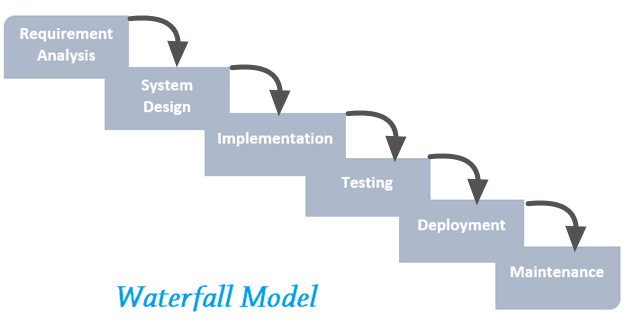
\includegraphics[width=\textwidth]{water}

\end{center}
\caption{Waterfall Model}
\end{figure}


In Waterfall Model phases are executed sequentially, in linear way. The project begins with a steady set of requirements that are non-changeable in time. The system is developed progressively and the business user is involved only in the early phases of the development. 
One of the advantages of the Waterfall Model is that it is easy to manage, with a set of requirements and the plan of execution both defined at the beginning of the project. The disadvantage of such model is that it contains a strict sequence of activities, which results in low cost of errors in beginning stages but very high importance and cost corrections in the later phases. Therefore this model can only be used when it is possible to precisely define the requirements at the beginning of the project.\cite{D}
 

\subsection{Argumentation}

The reasoning behind the choice of this particular development model is presented below:
\begin{itemize}
\item The sequential order of phases were aligned with the organized schedule of the development of the Engineering Thesis

\item Fixed set of requirements, known as the initial requirements were submitted by team to the Faculty and could not be changed later
\item Easy management of the work in the Waterfall Model is facilitating the work of the team
\item The use of this particular model was highly recommended by the coordinators of the Group Project and the supervisor of the thesis \cite{E}
 
\end{itemize}




% ----------------------- Systeem Architecture ------------------


\chapter{System Architecture}



\section{Software Architectural Pattern}

To facilitate the design of classes, the project team has decided to follow an already established software architectural pattern. A pattern of choice was the Model–View–Controller (MVC) Pattern.
The MVC pattern is used to separate a given application into three interconnected parts. The reason for doing that is to separate internal representations of information from the ways information is presented to, and accepted from, the user. The three parts composing the MVC model are: 
\begin{itemize}
\item Model – A model is a representation of an object carrying data. It can also have logic to update controller if its data changes.
\item View – A view represents the visualization of the data that model contains visible to the user.
\item Controller – A controller acts on both model and view. It controls the data flow into model object and updates the view whenever data changes. It keeps view and model separate. \cite{F} \cite{G}
 
 
\end{itemize}
\begin{figure}[h!]

\begin{center}

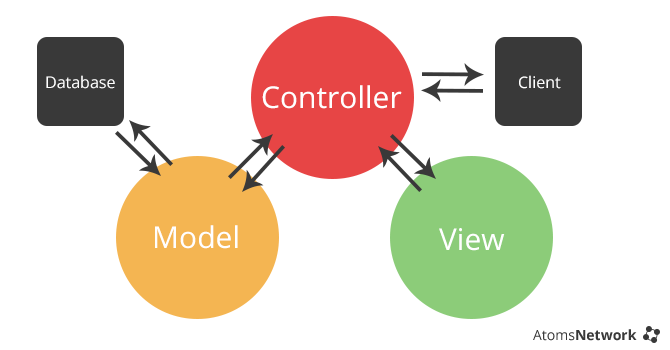
\includegraphics[width=\textwidth]{mvc}

\end{center}
\caption{MVC Pattern}
\end{figure}


The use of the MVC model has been very helpful while designing the division into projects’ classes. The Model, View and Controller Classes were designed for each element of the User Interface element.  Additionally, the database objects are handled by Servlet (classes taking an article from http POST and passing it to JDBC), DAO (classes responsible for the communication with database) and Query (classes to parse SQL) classes. These classes will be discussed in detail in the further chapters.

\section{Backend Architectural Patterns}

The L.I.M.E. application includes some more architectural patterns. Precisely chosen patterns make overall architecture strong and well built. The description of these backend architectural patterns will be provided in this section. 

\subsection{Data Access Object Pattern}

Data access object (DAO) is an object that provides an abstract interface to some type of database or other persistence mechanism. By mapping application calls to the persistence layer, the DAO provides some specific data operations without exposing the details of the database. This isolation supports the single responsibility principle. It separates the data access the application needs, in terms of domain-specific objects and data types (the public interface of the DAO), from how these needs can be satisfied with a specific DBMS, database schema, etc. (the implementation of the DAO).
The most important fact and advantage is the relatively simple and rigorous separation between two important parts of an application that can but should not know anything of each other, and which can be expected to evolve frequently and independently. Changing business logic can rely on the same DAO interface, while changes to persistence logic do not affect DAO clients as long as the interface remains correctly implemented. All details of storage are hidden from the rest of the application. Thus, possible changes to the persistence mechanism can be implemented by just modifying one DAO implementation while the rest of the application isn't affected.\cite{H}
The L.I.M.E. application implements one template parent interface with methods which are used by all DAO classes, this class being IBasicCrudRepository which extends Hibernate CrudRepository and inherits from it all CRUD database operations. Singular DAO classes implement service-specific methods which are defined this DAO interface. 
 

\subsection{Plain Old Java Object}

Plain old Java object (POJO) is an ordinary Java object, not bound by any special restriction and not requiring any class path. 
The main aim of the POJO classes is to differentiate business logic from database entity. It makes code cleaner and easier to read and understand.

\begin{figure}[h!]

\begin{center}

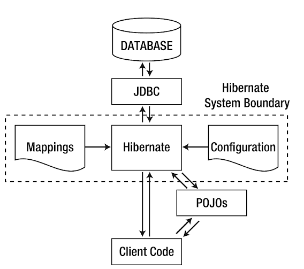
\includegraphics[scale=1]{pojo}

\end{center}
\caption{Plain Old Java Object in Backend Architecture}
\end{figure}
The POJO phenomenon has most likely gained widespread acceptance because of the need for a common and easily understood term that contrasts with complicated object frameworks. 
 

The L.I.M.E application implements POJO classes for all existing entity classes. Those classes are free from frameworks and complicated annotations. There is an implemented object mapper, which maps directly from Entity to POJO classes.



\subsection{Dependency Injection}

Dependency Injection is a broader version of ‘inversion of control’ (IoC) principle. It relates to the way in which an object obtains references its dependencies - the object is passed to its dependencies through constructor arguments or after construction through setter methods or interface methods. It is called dependency injection since the dependencies of an object are 'injected' into it. The term dependency is a little misleading here, since it is not a new 'dependency' which is injected but rather a 'provider' of that particular capability. For example, passing a database connection as an argument to a constructor instead of creating one internal would be categorized as dependency injection.
The pattern seeks to establish a level of abstraction via a public interface and to remove dependencies on components by supplying a 'plugin' architecture. This means that the individual components are tied together by the architecture rather than being linked together themselves. The responsibility for object creation and linking is removed from the objects themselves and moved to a factory.


\begin{figure}[h!]

\begin{center}

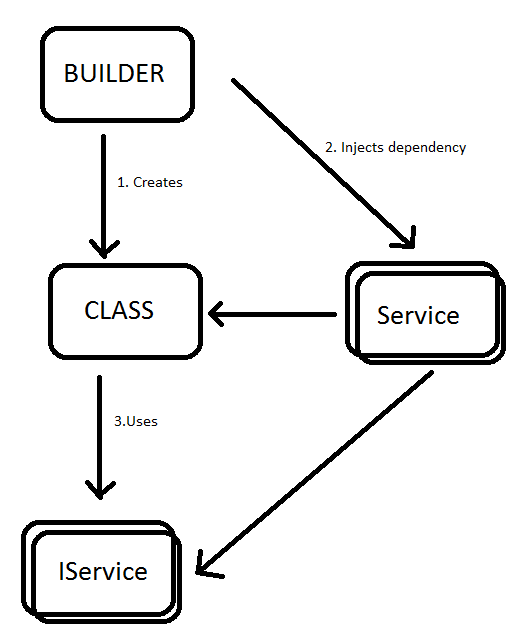
\includegraphics[scale = 1]{dependency}

\end{center}
\caption{Dependency Injection}
\end{figure}
The main advantage of Dependency Injection is fact that there is only one instance of each object shared through multiple controllers. What is more, it allows a client the flexibility of being configurable. Only the client's behavior is fixed. The client may act on anything that supports the intrinsic interface the client expects.
Dependency injection can be used to externalize a system's configuration details into configuration files, allowing the system to be reconfigured without recompilation. Separate configurations can be written for different situations that require different implementations of components. This includes, but is not limited to, testing. \cite{I}
The L.I.M.E. application uses Spring dependency injection. There are bean services, which implement the domain logic. Each service implements interface defining the methods. Interfaces and services correspond to Hibernate’s entities and fulfill the needs of application logic. Interface beans are auto wired into the REST controllers.

\subsection{RESTful API}

REpresentational State Transfer (REST) is an architectural style that defines a set of constraints and properties based on HTTP. REST-compliant web services allow the requesting systems to access and manipulate textual representations of web resources by using a uniform and predefined set of stateless operations. Other kinds of web services, such as WSDL and SOAP, expose their own arbitrary sets of operations.
In a RESTful web service, requests made to a resource's URI will elicit a response that may be in XML, HTML, JSON, or some other format. The response may confirm that some alteration has been made to the stored resource, and the response may provide hypertext links to other related resources or collections of resources. When HTTP is used, as is most common, the operations available are GET, POST, PUT, DELETE, and other predefined CRUD HTTP methods. \cite{J}


\begin{figure}[h!]

\begin{center}

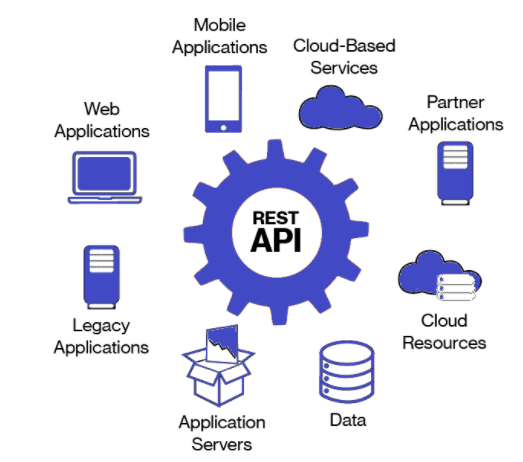
\includegraphics{rest}

\end{center}
\caption{RESTful API}
\end{figure}
The L.I.M.E. application implements RESTful controllers which are used to communicate with a client part of application. They communicates with a JSON body type. CRUD methods like PUT, DELETE, POST, GET are used to make action more readable and indicate what exactly is being done. There are Controllers corresponding to each view in a client part. 

% ----------------------- Technical Analysis ------------------


\chapter{Technical Analysis}


\section{Client-Server Architecture}
Client/server architecture is a producer/consumer computing architecture where the server acts as the producer and the client acts as a consumer. The server houses and provides high-end, computing-intensive services to the client on demand.
The L.I.M.E. application implements client-service architecture. There are 2 applications in the project:
\begin{enumerate}
\item Server implemented in JAVA,
\item GUI implemented with AngularJS
\end{enumerate}
Communication between client and server is done with RESTful API. Server accepts request from authenticated users sent from GUI. Then the server process the request, saves the data in the database and sends the answer back to the client.


\begin{figure}[h]

\begin{center}

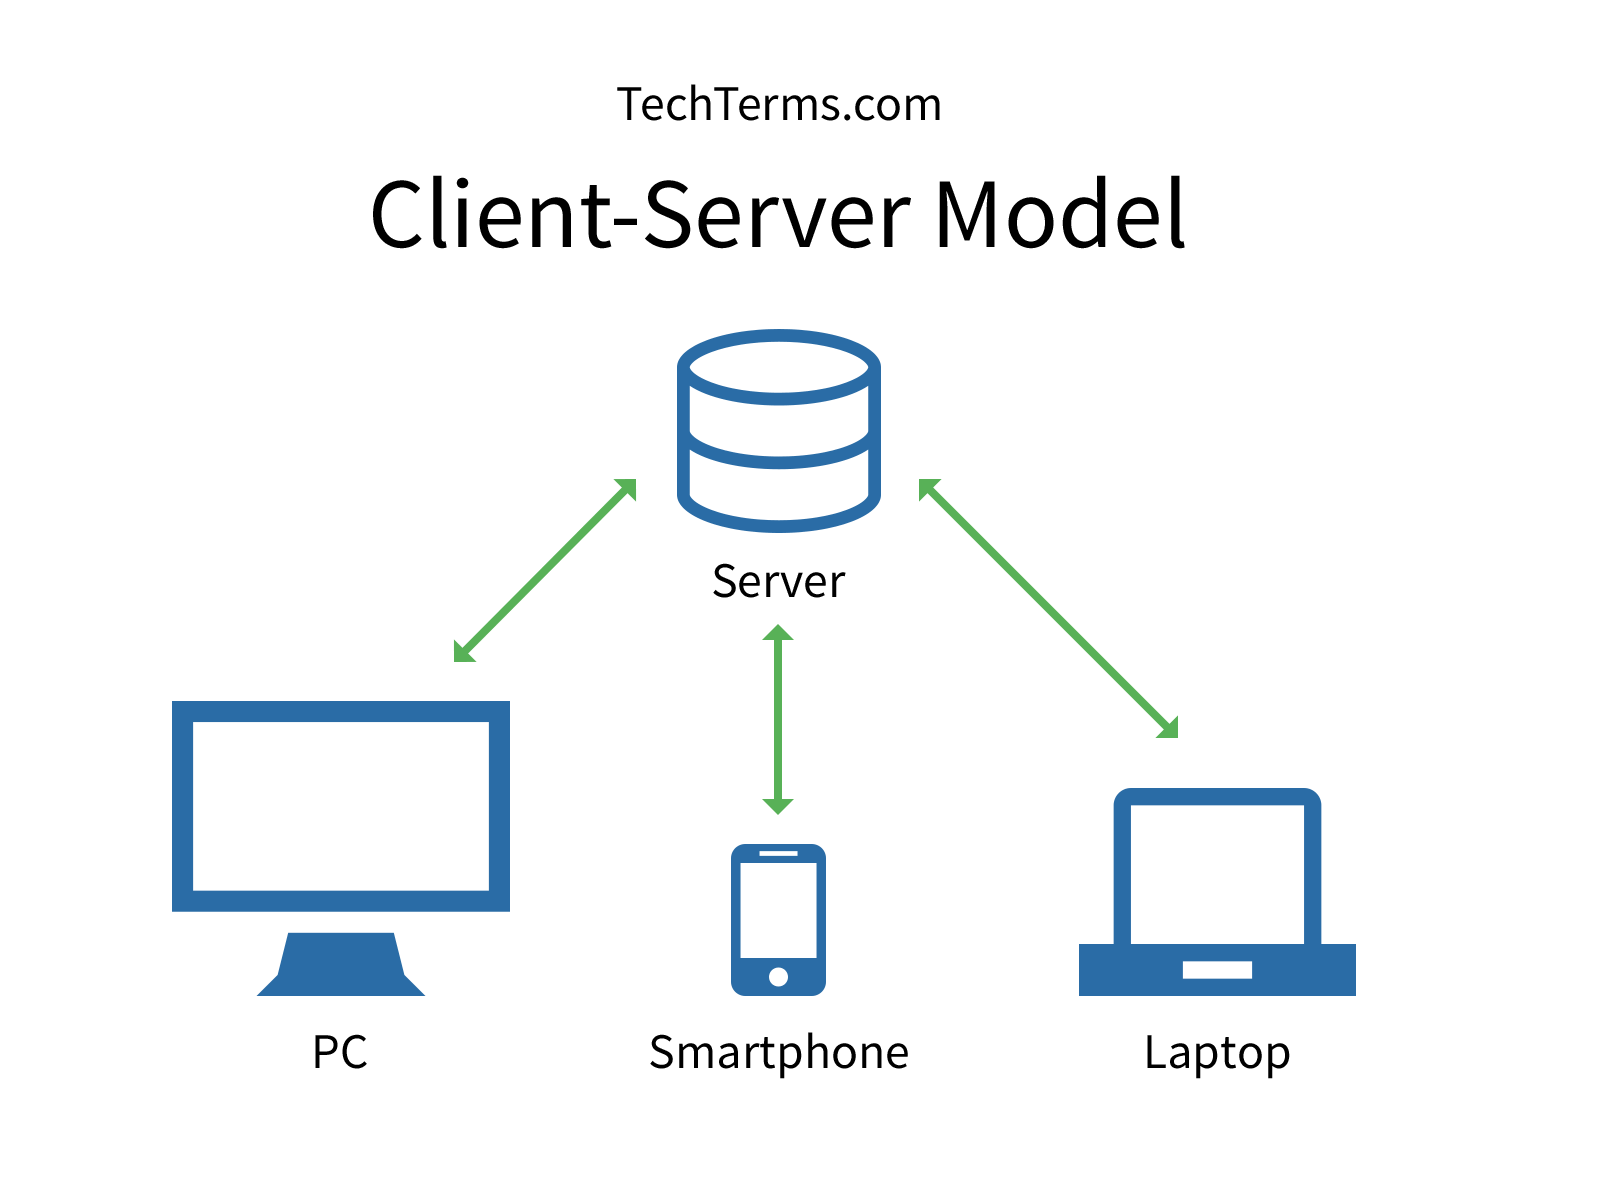
\includegraphics[scale = 0.5]{CS}

\end{center}
\caption{Client-Server Architecture}
\end{figure}

\section{Login}
The L.I.M.E. application has got a system to recognize users and their roles. It is implemented using Spring Security. When the user logs in, the GUI application sends login request to server and the server application checks whether the user exists and which role does he have. As a response, the server passes the authorization data which is valid for 12 hours (session timeout). Each request from GUI to Server contains a header with the authorization data, so server can recognize which user sends request and if he has an appropriate role.
\section{Program Interface}

The User Interface of L.I.M.E application consists of a top menu with the logo and the name of the system, which is common for all views. On the right side of the menu, there is a smaller dropdown menu with login and reset password options. On the bottom of the page there is a footer. After logging in, the login dropdown menu switches to user account options and on the left side of the page a side menu appears with different subpages available, depending on a role the user has. In the whole application there are following views (subpages) available:

\begin{enumerate}
\item Login page:
\begin{enumerate}
\item input boxes for username and password
\item login button
\end{enumerate}
\item Password recovery page:
\begin{enumerate}
\item inputs for email and email confirmation
\item reset button
\end{enumerate}
\item Edit account page:
\begin{enumerate}
\item inputs for name, surname, email address, username and password
\item edit button
\end{enumerate}
\item Login welcome page:
\begin{enumerate}
\item welcome banner with logout button
\end{enumerate}
\item Welcome page:
\begin{enumerate}
\item banner with information about application
\end{enumerate}
\item Resources page:
\begin{enumerate}
\item table displaying resources with name, image, description, quantity and unit.
\item buttons for viewing details, editing and deleting each resource
\item button for adding new resource
\item search field for filtering resources by name 
\end{enumerate}
\item Products page:
\begin{enumerate}
\item table displaying product with name, image, description, expected value and unit.
\item buttons for viewing details, editing and deleting each product
\item buttons for viewing and editing formula of each product
\item button for adding new resource
\item search field for filtering resources by name
\end{enumerate} 
\item Orders page:
\begin{enumerate}
\item checkbox list with resources names and input for quantity of given resource
\item send button for sending order to suppliers
\item switch for turning auto orders on or off
\end{enumerate}
\item Report generation page for resources/products:
\begin{enumerate}
\item list of resources/products with checkboxes
\item list of charts types with radio buttons
\item input for start date
\item input for number of days 
\item input for email of  report receiver
\item send report button for sending it by an email
\item generate report button for displaying it on the current page
\end{enumerate}
\item Report prediction page for resources/products:
\begin{enumerate}
\item list of  checkboxes with resources/products names
\item list of radio buttons with charts types
\item input for start date
\item input for number of days
\item input for number of days of forecast
\item email of receiver
\item send report button for sending it by an email
\item generate report button for displaying it on the current page
\end{enumerate}
\item Categories page for resources/products:
\begin{enumerate}
\item table displaying resources/products categories
\item button for editing and deleting each category
\item button for adding new category
\end{enumerate}
\item Notifications page: 
\begin{enumerate}
\item table displaying resources with its critical values and notification status
\item buttons for editing notifications of each resource separately
\item switch for turning notifications for all resources on or off
\end{enumerate}
\item Suppliers page:
\begin{enumerate}
\item table displaying suppliers with name, telephone, city, country,  postal code, street and email address 
\item buttons for viewing details, editing and deleting each supplier
\item button for adding new supplier
\item search field for filtering suppliers by all displayed values
\end{enumerate}
\item Jobs page:
\begin{enumerate}
\item table displaying jobs with product name, description, start and end date, result value and username
\item button for adding new job
\end{enumerate}
\item Users page:
\begin{enumerate}
\item table displaying users with name, surname, username, email address and roles
\item buttons for viewing details, editing and deleting each user
\item button for adding new user
\item search field for filtering users by all displayed values
\end{enumerate}
\end{enumerate}

Whenever a user presses a view button next to the resource or product, a pop-up modal opens with more detailed information about selected item such as its quantity. Similarly, an edit modal also displays information about selected item, but in the form of input boxes, so there is a possibility to modify them. Clicking delete button next to a resource or product results in showing a confirmation dialog.\\ \\

The main requirement concerning UI of the L.I.M.E. application was to make the interface user friendly. It has been fulfilled by implementing pleasant looking and easy to navigate GUI. Placement of main components is quite standard – account settings in top right corner, main menu on the left side panel – which makes the interface intuitive for the user. Throughout the whole application there are used common UI elements and the pattern in layout can be noticed. The purpose of that is to make user feel more comfortable and consequently make him use application more efficiently. Interface is also simple in design, there are no unnecessary elements and the language used on labels is rather clear and understandable. Another important aspect is efficient error handling. Whenever application comes across an error, it informs the user about the encountered problem and gives the user a possibility to report a bug to the developers, by sending an email to the given address. As the result application becomes easy to troubleshoot – user can contact the support and that support will resolve the issue. \\ \\

The core functionality of L.I.M.E. application is user specific context i.e. user account. Authorization mechanism consists of two core components: client-side application and backend-side authorization provider. From the business perspective client-side application is responsible for retrieving user data, validation and sending data to authorization provider in secure way. First two elements are customized, out of the box functionalities of used technologies. Sending sensitive data is realized by encoding HTTP request data with Base64 encoder. After successful logging in encoded credentials are used in all further requests in HTTP Authorization header. It allows backend to intercept all incoming movement with checking if specific request is coming from authorized user.\\ \\


\section{System Classes}

The L.I.M.E Application is composed with the following packages, and the packages contain the following classes and interfaces:

\begin{enumerate} 
\item Lime 
\begin{enumerate} 
\item \textbf{LimeApplication} Springboot launch class for the L.I.M.E. application.
\end{enumerate}
\item Api 
\begin{enumerate} 
\item \textbf{GlobalExceptionHandlingControllerAdvice} Performs exception handling for all REST API controllers.
\end{enumerate} 
\item ClassModels 
\begin{enumerate} 
\item \textbf{DrawSeries} The class for plotting Time Series into a Chart
\item \textbf{TimeSeries} The class of Time Series
\end{enumerate} 
\item Config 
\begin{enumerate} 
\item \textbf{SecurityConfiguration} Spring Security configuration class.

\item \textbf{StorageProperties} Properties which indicate location of resources (images), taken out from application.yml.
\item \textbf{SwaggerConfig} Main configuration class to enable the Swagger UI frontend.
\end{enumerate} 

\item Controller 
\begin{enumerate} 
\item \textbf{BaseController} Abstract controller - provides invalid request exception handler.
\item \textbf{DevController} REST Controller used only for test purposes, includes a database populator.
\item \textbf{FileUploadController} REST Controller for File operations.
\item \textbf{ForecastController} REST Controller for Forecast operations.
\item \textbf{FormulaController} REST Controller for Formula operations.
\item \textbf{JobController} REST Controller for Job operations.
\item \textbf{OrderController} REST Controller for Order operations.
\item \textbf{ProductCategoryController} REST Controller for Product operations.

\item \textbf{ProductController} REST Controller for Product operations.
\item \textbf{ReportController} REST Controller for Report operations.
\item \textbf{ResourceCategoryController} REST Controller for Resource operations.
\item \textbf{ResourceController} REST Controller for Resource operations.
\item \textbf{SupplierController} REST Controller for Supplier operations.
\item \textbf{UserController} REST Controller for User operations.

\end{enumerate} 

\item Dao 
\begin{enumerate} 
\item \textbf{IBasicCRUDRepository<T,ID extends java.io.Serializable>} The interface
    Basic crud repository - interface for parents of all Spring repositories.
\item \textbf{IFormulaDAO} The interface for Formula dao.
\item \textbf{IJobDAO} The interface for Job dao.

\item \textbf{IProductCategoryDAO} The interface for Product category dao.
\item \textbf{IProductDAO} The interface for Product dao.
\item \textbf{IResourceCategoryDAO} The interface for Resource category dao.
\item \textbf{IResourceDAO} The interface for Resource dao.

\item \textbf{IRoleDAO} The interface for Role dao.

\item \textbf{ISupplierDAO} The interface for Supplier dao.
\item \textbf{IUserDAO} The interface for User dao.

\end{enumerate} 
\item Exception 
\begin{enumerate} 

\item \textbf{AlreadyExistsException} Exception thrown when an entity already exists (the new entity does not have at least one unique field).
\item \textbf{ForbiddenException} Exception thrown when e.g. an authentication attempt is not allowed with the given credentials (no details returned).
\item \textbf{IllegalDataException} Exception thrown when the given data is not valid in the current context.
\item \textbf{InvalidRequestException}Exception thrown when a request is invalid in the current context.
\item \textbf{NotAcceptableException} Exception thrown when given data is not acceptable.
\item \textbf{NotFoundException} Exception thrown when an entity is not found where expected.
\item \textbf{OperationNotAllowedException} Exception thrown when a contract management API call is not allowed.
\item \textbf{ServiceUnavailableException} Exception thrown when the Service is unavailable.
\item \textbf{StorageException} Exception thrown when a storage error occurs.

\item \textbf{StorageFileNotFoundException} Exception thrown when the file is not found.
\item \textbf{UnprocessableEntityException} Exception thrown when an entity contains validation errors.

\end{enumerate} 
\item Model 
\begin{enumerate}
 
\item \textbf{CustomUserDetails} The implementation of a Spring users credentials storage.
\item \textbf{Formula} Model representation of a formula used in Lime.
\item \textbf{Job} Model representation of a job created by Lime user.
\item \textbf{Product} Model representation of a product added in Lime.
\item \textbf{ProductCategory} Model representation of a product category.
\item \textbf{Resource} Model representation of a resource used in Lime.
\item \textbf{ResourceCategory} Model representation of a resource category.
\item \textbf{Role} Model representation of a user role in Lime.
\item \textbf{Supplier} Model representation of a supplier in Lime.
\item \textbf{User} Model representation of user of Lime.

\end{enumerate} 
\item Pojo 
\begin{enumerate} 
\item \textbf{BasicPOJO} Plain old java object representation of each object.
\item \textbf{FormulaPOJO} Plain old java object representation of Formula objects.
\item \textbf{JobPOJO} Plain old java object representation of Job objects.
\item \textbf{ProductCategoryPOJO} Plain old java object representation of Product category objects.
\item \textbf{ProductPOJO} Plain old java object representation of Product objects.
\item \textbf{ResourceCategoryPOJO} Plain old java object representation of Resource category objects.

\item \textbf{ResourcePOJO} Plain old java object representation of Resource objects.

\item \textbf{RolePOJO} Plain old java object representation of Role objects.
\item \textbf{SupplierPOJO} Plain old java object representation of Supplier objects.
\item \textbf{UserPOJO} Plain old java object representation of User objects.

\end{enumerate} 
\item Service 
\begin{enumerate} 

\item \textbf{IBasicCRUDService} The interface - parent of all crud services.
\item \textbf{IForecastService} The interface Forecast service.
\item \textbf{IFormulaService} The interface Formula service.
\item \textbf{IJobService} The interface Job service.
\item \textbf{IMailService} The interface Mail service.
\item \textbf{INotificationService} The interface Notification service.
\item \textbf{IProductCategoryService} The interface Product category service.
\item \textbf{IProductService} The interface Product service.
\item \textbf{IReportService} The interface Report service.
\item \textbf{IResourceCategoryService} The interface Resource category service.
\item \textbf{IResourceService} The interface Resource service.
\item \textbf{IRoleService} The interface Role service.
\item \textbf{ISmoothingService} The interface Smoothing service.
\item \textbf{IStorageService} The interface Storage service.
\item \textbf{ISupplierService} The interface Supplier service.
\item \textbf{ITimeSeriesService} The interface Time series service.
\item \textbf{IUserService} The interface User service.

\end{enumerate} 
\begin{enumerate} 
\item \textbf{BasicCRUDService} Implementation of parent of CRUD services - implements methods which all child classes use.
\item \textbf{CustomUserDetailsService} Service that provides all methods needed to manage Custom objects.
\item \textbf{ForecastService} Service that provides all methods needed to manage Forecast objects.
\item \textbf{FormulaService} Service that provides all methods needed to manage Formula objects.
\item \textbf{JobService} Service that provides all methods needed to manage Job objects.
\item \textbf{MailService} Service that provides all methods needed to manage Mail objects.
\item \textbf{NotificationService} Service that provides all methods needed to manage Notification objects.
\item \textbf{ProductCategoryService} Service that provides all methods needed to manage Product Category objects.
\item \textbf{ProductService} Service that provides all methods needed to manage Product objects.


\item \textbf{ReportService} Service that provides all methods needed to manage Report objects.
\item \textbf{ResourceCategoryService} Service that provides all methods needed to manage Resource Category objects.
\item \textbf{ResourceService} Service that provides all methods needed to manage Resource objects.
\item \textbf{RoleService} Service that provides all methods needed to manage Role objects.

\item \textbf{SmoothingService} Service that provides all methods needed to manage Smoothing objects.
 \item \textbf{StorageService} Service that provides all methods needed to manage Storage objects.

\item \textbf{SupplierService} Service that provides all methods needed to manage Supplier objects.
\item \textbf{TimeSeriesService} Service that provides all methods needed to manage Time Series objects.

\item \textbf{UserService} Service that provides all methods needed to manage User objects.


\end{enumerate} 
\item Tools
\begin{enumerate} 
\item \textbf{ParseTools} Contains tools for parsing various objects.
\item \textbf{StartUpPopulator} Contains a populator of a database for production application startup.

\item \textbf{TSGenerator} Contains a generator of sample Time Series.



\end{enumerate}
\end{enumerate}

The attached description of classes is obviously a very brief one. Due to the amount of classes in this application it could not be possible to contain all of the methods as well or even a longer description. \\
The interface, class, enum, method descriptions and hierarchy can be found and browsed in "Classes and method report" by launching index.html

\section{Database Design}
 

\begin{figure}[hb!]

\begin{center}

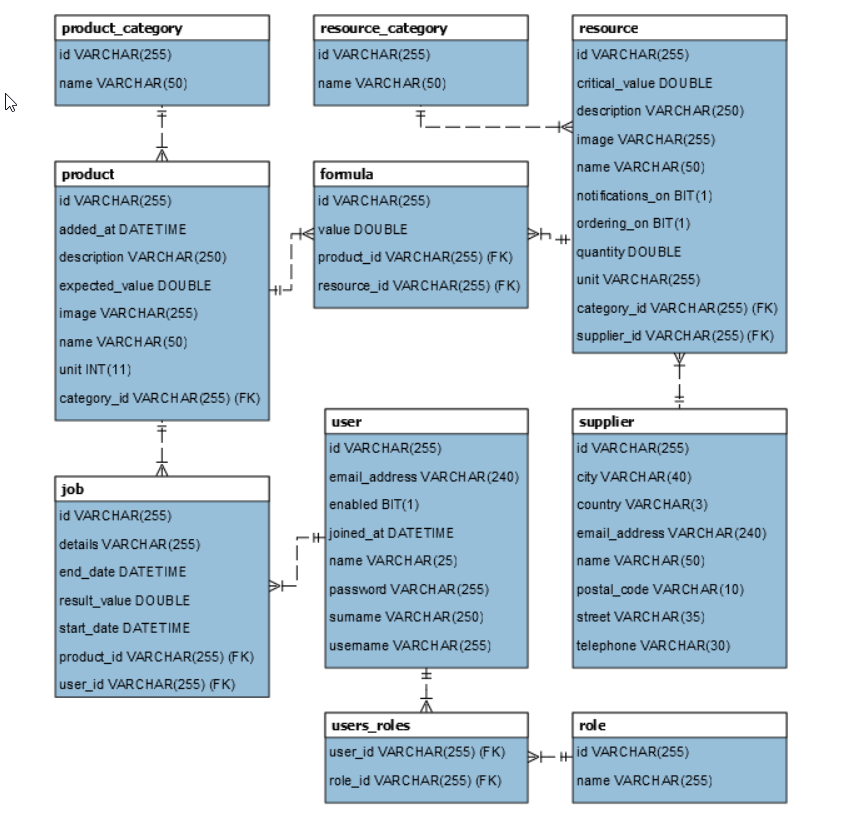
\includegraphics{DB4}

\end{center}
\caption{Database Design}
\end{figure}

The database consists of the following tables:

\begin{enumerate}
\item \textbf{Product} Stores information about products (complex structures of resources) with their properties:
\begin{enumerate}
\item \textbf{Product ID} ID of a product
\item \textbf{Added At} Date of adding a product to a database
\item \textbf{Description} Description of a product
\item \textbf{Expected Value} Expected value - how much of a product shall be obtained after production
\item \textbf{Image} Image for this product
\item \textbf{Name} Name of a product
\item \textbf{Unit} Unit of a measurement
\item \textbf{Category ID} Assigns a product to a category
\end{enumerate}

\item \textbf{Product Category} Stores information about product categories: its name and ID

\item \textbf{Job} Logs the jobs performed by the user and the following details:
\begin{enumerate}
\item \textbf{Job ID} ID of a job
\item \textbf{Details}More details about the job
\item \textbf{Result Value} Result value - how much of a product was actually obtained after production
\item \textbf{Start Date} Start date of a job
\item \textbf{End Date} End date of a job
\item \textbf{Product ID} ID of a product that resulted from this job
\item \textbf{User ID} Assigns a job to a user which have performed it
\end{enumerate}

\item \textbf{User} The table stores properties of every user of the system, such as:
\begin{enumerate}
\item \textbf{User ID} ID of a user
\item \textbf{Email address} Email address of this user
\item \textbf{Enabled} Indicates if this an active user of the system
\item \textbf{Joined At} Date of joining the system
\item \textbf{Name} Given Name
\item \textbf{Surname} Surname
\item \textbf{Username} Username chosen by the user
\item \textbf{Password} User's password in encrypted form
\end{enumerate}

\item \textbf{User Roles} Assigns users to their roles (resolves the many-to-many relationship)

\item \textbf{Role} Stores each role with its name and ID

\item \textbf{Formula} Resolves the many-to-many relation between resources and product, represents the quantity of resources used to make a product
\begin{enumerate}
\item \textbf{Formula ID} ID of a formula
\item \textbf{Product ID} ID of a product
\item \textbf{Resource ID} ID of a resource
\item \textbf{Value} The amount of a given resource needed to make the given product
\end{enumerate}

\item \textbf{Resource} Stores information about a basic laboratory resource and its properties, such as:
\begin{enumerate}
\item \textbf{Product ID} ID of a resource
\item \textbf{Description} Description of a resource
\item \textbf{Image} Image for the resource
\item \textbf{Name} Name of a resource
\item \textbf{Critical Value} critical value - how much of a resource shall be left for the notifications of the low level of resource to be triggered
\item \textbf{Notifications On} Are the notifications about the low level of the resource turned on
\item \textbf{Ordering On} Indicates if automatic ordering of the resource is turned on
\item \textbf{Quantity} the amount of the resource at the storage at the moment
\item \textbf{Unit} Unit of a measurement
\item \textbf{Category ID} Assigns a resource to a category
\item \textbf{Supplier ID} Assigns a resource to a supplier
\end{enumerate}

\item \textbf{Resource Category} Stores information about resource categories: its name and ID

\item \textbf{Supplier} Stores data about suppliers assigned to each resources
\begin{enumerate}
\item \textbf{Supplier ID} ID of a supplier
\item \textbf{Email address} Email address of this supplier
\item \textbf{Name} Name of the supplier
\item \textbf{Street} Address of the supplier: street name and number
\item \textbf{City} Address of the supplier: City
\item \textbf{Postal Code} Address of the supplier: Postal Code
\item \textbf{Country} Address of the supplier: Country
\item \textbf{Telephone} Telephone number of this supplier
\end{enumerate}

\end{enumerate}

\section{Forecast}

The prediction of the future values of production of products and usage of resources is one of the key features of the application.
The data collected from the application are in the form time series:
\begin{definition}[Time Series]
The expression \textit{time series data}, or \textit{time series} usually refers to a set of observations collected sequentially in time. These observations could have been collected at equally spaced time points. In this case we use the notation $y_t$ with ($t$ = ..., -1, 0, 1, 2, ...), i.e., the set of observations is indexed by $t$, the time at which observation was taken.
\end{definition}

There are many known models for the prediction of time series: starting from the simplest ones as predicting by using average or moving average, through exponential smoothing models and regression models to the most sophisticated models like ARMA, ARIMA models.
Many known models for time series prediction were researched, until we found the one that was appropriate to use in the application. The Exponential Smoothing Model was chosen for the following reasons:
\begin{enumerate}
\item The set of variables is rather small and rather simple therefore there was no reason to use more sophisticated methods.
\item The prediction model was to be implemented from scratch. Many more complicated methods could have been imported into the application using libraries, but the decision was made that it would be more challenging for the project to take one of the less complicated methods and then the project team implemented every step of it on their own.
\item The Holt's Linear Exponential Smoothing Method was chosen in particular because we have noticed that the data may possess a trend, as the laboratory production grows over time. \cite{K}
\end{enumerate}

\subsection{Holt's Linear Exponential Smoothing Method}

Holt developed a linear exponential smoothing method to allow forecasting of data with trends. The forecast for Holt's linear exponential smoothing is found using two smoothing constants $\alpha$ and $\beta$ (with values between 0 and 1), and three equations

\begin{equation}\label{Holt's Exponential smoothing 1}
L_t = \alpha Y_t + (1 - \alpha) (L_{t-1} + b_{t-1})
\end{equation}
\begin{equation}\label{Holt's Exponential smoothing 2}
b_t = \beta (L_t - L_{t-1}) + (1 - \beta) b_{t-1}
\end{equation}
\begin{equation}\label{Holt's Exponential smoothing 3}
F_t+m = L_t - b_t m
\end{equation}

Here, $L_t$ denotes an estimate of the level of the series at time $t$ and $b_t$ denotes an estimate of the slope of the series at time $t$. Equation 6.1 adjusts $L_t$ directly for the trend of the previous period, $b_{t-1}$, by adding it to the last smoothed value, $L_{t-1}$. This helps to bring $L_t$ to the approximate trend of thew current data value. Equation 6.2 then updates the trend, which is expressed as the difference between the last two smoothed values. This is appropriate, because if there is a trend in the data, new values should be higher or lower than the previous one. Since they may be some randomness remaining, the trend is modified by smoothing with $\beta$ the trend in the last period $L_t - L_{t-1}$ and adding that to the previous estimate of the trend multiplied by $ (1 - \beta)$. Finally, equation 6.3 is used to forecast ahead. The trend $b_t$ is multiplied by the number of periods ahead to be forecast, $m$ and added to the base value $L_t$.
\begin{definition}[Mean Squared Error]
If $Y_t$ is the actual observation for time period $t$ and $F_t$ is the forecast for the same period, then the error is defined as:
\begin{equation}\label{Error}
e_t = Y_t - F_t
\end{equation}
Usually $F_t$ is calculated using data $Y_1$, ..., $Y_{t-1}$. it is one- step forecast because it is forecasting one period ahead of the last observation used in the calculation. Therefore $e_t$ can be described as a \textit{one-step forecast error}. It is the difference between the observation $Y_t$ and the forecast made using all the observation but not including $Y_t$. 
If there are observations and forecasts for $n$ time periods, then there will be $n$ error terms, and the following standard statistical measure Mean Square Error can be defined:
\begin{equation}\label{Mean Squared Error}
MSE = 1/n \sum_{t=1}^{n} e_t^{2} 
\end{equation} \cite{L}

\end{definition}
The $\alpha$ and $\beta$ coefficients used for the calculation of smoothing are being optimized so that the Mean Squared Error is minimized.



% ----------------------- Experimental Evaluation ------------------

\chapter{Post Execution Documentation}

In this section the final application was tested against the set of initial requirements. For every requirement given in Chapter 3, discussed is how the particular requirement is implemented in the application.

\section{Evaluating Functional Requirements}

The following sections will discuss how the functional requirements were implemented, separately for every group of users (Administrator, Manager and User)

\subsection{Administrator}

\begin{longtable}{|p{4cm}|p{12cm}|}
\caption[Evaluating Functional Requirements for Administrator]{Evaluating Functional Requirements for Administrator}
\label{Evaluating Functional Requirements for Administrator}
\centering
\tabularnewline

\hline
\textbf{Functional \mbox{Requirement}} & \textbf{Implementation} \\ \hline
Log in to the system and change his & L.I.M.E. application recognize users and its roles. It is implemented using Spring security. Password can be changed by the administrator of the system. \\ \hline
Create, modify and remove an account in the system, modify its roles & Administrator can create account via Manage Users view. It is possible to choose from 3 roles: administrator, manager and staff. It is also possible to edit or remove an account in the same view. \\ \hline
View, create, modify and remove resources and products & Administrator can create products and resources in products view and resources view respectively. It is also possible to modify and remove objects in the same view. \\ \hline
View, create, modify and remove groups of resources and products & Administrator can create groups of products and resources choosing products or resources in manage groups respectively. It is also possible to modify and remove objects in the same view. \\ \hline
View, create, modify formula of the product & Administrator can create formula for the given product choosing resources and putting the needed value. It is possible to create and modify formula in products view. \\ \hline
Define, generate and send a report & Administrator can define and generate report depending on date range and resources or products. It can be done in reports view, product and resource subpage respectively. \\ \hline
Define, generate and send a prediction & Administrator can define and generate prediction depending on date range and resources or products. It can be done in prediction view, product and resource subpage respectively. \\ \hline
Define notifications, turn notifications on & Administrator can define critical value of the resource in notifications view. He will be notified via email that the selected resource exceed critical value. The notifications can be set on/off separately for each object or for all with one button. \\ \hline
Create job, declare time range of the job & Administrator can create job, choose the product which resulted from the job and declare time range within which the job was done. It can be done in job view. \\ \hline
Order resources, turn on/off automatic ordering & Administrator can order the resources - supplier will be notified with a mail. It is also possible to group resources and send one order. It is possible to turn on/off automatic orders - an order will performed when the resource exceed critical value. It can be done in manage orders view. \\ \hline


\end{longtable}

\subsection{Manager}

\begin{longtable}{|p{4cm}|p{12cm}|}
\caption[Evaluating Functional Requirements for Manager]{Evaluating Functional Requirements for Manager}
\label{Evaluating Functional Requirements for Manager}
\centering
\tabularnewline

\hline
\textbf{Functional \mbox{Requirement}} & \textbf{Implementation} \\ \hline

Log in to the system & L.I.M.E. application recognize users and its roles. It is implemented using Spring security. Password can be changed by the administrator of the system. \\ \hline
View, create, modify and remove resources and products & Manager can create products and resources in products view and resources view respectively. It is also possible to modify and remove objects in the same subpage. \\ \hline
Define, generate and send a report & Manager can define and generate a report depending on date range and resources or products chosen. It can be done in reports view, product and resource subpage respectively. \\ \hline
Define, generate and send a prediction & Manager can define and generate prediction concerning a selected date range and resources or products. It can be done in prediction view, product and resource subpage respectively. \\ \hline
Define notifications, turn notifications on & Manager can define critical value of the resource in notifications view. He will be notified via email that the selected resource exceed critical value. The notifications can be set on/off separately for each object or for all with one button. \\ \hline
Order resources, turn on/off automatic ordering & Manager can order the resources – the supplier will be notified via mail. It is possible to group resources and send one order. It is also possible to turn on/off automatic orders - an order will be performed when the resource exceed critical value. It can be done in manage orders view. \\ \hline
Create job, declare time range of the job & Manager can create job, choose the product which resulted from the job and declare time range within which the job was done. It can be done in job view. \\ \hline



\end{longtable}

\subsection{User}

\begin{longtable}{|p{4cm}|p{12cm}|}
\caption[Evaluating Functional Requirements for User]{Evaluating Functional Requirements for User}
\label{Evaluating Functional Requirements for User}
\centering
\tabularnewline

\hline
\textbf{Functional \mbox{Requirement}} & \textbf{Implementation} \\ \hline
Log in to the system & L.I.M.E. application recognize users and its roles. It is implemented using Spring security. Password can be changed by administrator of the system. \\ \hline
View, create, modify and remove resources and products & User can create products and resources in products view and resources view respectively. It is also possible to modify and remove objects in the same subpage. \\ \hline
Define, generate and send a report & User can define and generate a report depending on date range and resources or products chosen. It can be done in reports view, product and resource subpage respectively. \\ \hline
Define, generate and send a prediction & User can define and generate prediction concerning a selected date range and resources or products. It can be done in prediction view, product and resource subpage respectively. \\ \hline
Order resources & User can order the resources – the supplier will be notified via mail. It is possible to group resources and send one order. It can be done in manage orders view. \\ \hline
Create job, declare time range of the job & User can create job, choose the product which resulted from the job and declare time range within which the job was done. It can be done in job view. \\ \hline




\end{longtable}

\section{Evaluating Non-Functional Requirements}

Similarly, this section will discuss how the non-functional requirements were implemented

\begin{longtable}{|p{3cm}|p{7cm}|p{6cm}|}
\caption[Evaluating Non-Functional Requirements]{Evaluating Non-Functional Requirements}
\label{Evaluating Non-Functional Requirements}
\centering
\tabularnewline

\hline
\textbf{Area} & \textbf{Non-Functional Requirement} & \textbf{Implementation} \\ \hline
Usability & Application must be responsive. It must be working on PC, tablets and phones with resolution at least 720p. & GUI is implemented with responsive frameworks: Angular and bootstrap \\ \hline
Reliability & Application must be of type High Availability. It should be available
24/7, between 08:00 and 23:00. There could be service breaks during the week between 24:00 and 8:00. & Application is deployed on Heroku. The application is available 24/7 \\ \cline{2-3}
& Application must have quick restart in case of app machine failures. & It is possible to restart app with command: heroku restart \\ \hline
Recovery & Application must have daily database backup performed 24:00 and 08:00. & 
Database has default scheduled database dumps. It can be rescheduled in Heroku database configuration \\ \hline
Performance & Application should respond no longer than 3 seconds while strain being on level 100 queries per minute. & Application uses client server architecture. RESTful Api delivers much higher capacity. \\ \hline
Supportability & Documentation should contain instruction for recovery data from
database backup. & In the User Manual, there is a step by step description on how to perform a database backup, scheduling  and recovery. \\ \cline{2-3}
& Application should keep backward compatibility between the released versions. & With the future releases version, there will be database script provided, which will fill previous entries. \\ \hline
Security & Application must have user levels security. It shall not pass a user who has inappropriate privileges. & Application has implemented user service implemented with Spring security, which validates if the user exists and check for each REST endpoint if the user has appropriate privileges. \\ \hline

\end{longtable}




% ----------------------- Conclusions ------------------
\chapter*{Conclusions}


One of the most important goals of the thesis was to deliver software that will be used by the consumers of the market. Work began with a market research. The project team has received several proposals and chose the one that we considered the most appropriate for the subject of the engineering thesis. The decision was made to develop the ultimate system to manage the warehouse and human resources of the laboratory. The resulting project – L.I.M.E (Laboratory Internal Management Entity) was developed in line with market needs, being consulted with major consumers.\\ \\
At first, the project team has decided how the database will look like - what entities, relations and what type of the database will be used. That was the fundamental part of the application. This part of the project can be concluded as being completed perfectly. Even though there were a few minor changes but most of the original database project fulfilled needs of the application.\\ \\
Secondly, the project team had to develop the basic back-end parts of the application: connection with a database, user authentication and roles. Many additional features like database populator were developed additionally at this stage, for test purposes. \\ \\
Subsequently the project team has started to develop the client application. This was the hardest part of the project. It was difficult to write simultaneously front-end and back-end part of the application. There were many disagreements, and often the project team had to have long discussions before finally achieving the best solutions.\\ \\
Afterwards, when already most of the functionalities were implemented, the project team started to develop the features that are used by the most of the functionalities – reports, predictions, notifications. It required knowledge from the area of algorithms and mathematics. \\ \\
To develop the application, he top software technologies were. Server side is built with Java, Spring, SpringBoot, SpringSecurity and MySQL while the client side application was developed using AngularJS and Bootstrap. The communication between units was made with RESTful API. The well-known and widely used solutions helped the team to achieve final success. \\ \\
During the entire duration of the project, each progress in development was documented. Then, the documentation is essential for the project was written. The manual was delivered for the consumers, to help them understand how to properly use and take full advantage of L.I.M.E. \\ \\
Despite the many difficulties the project team has encountered and the fact that the completion of the project consumed about 40\% more time than was estimated, the results are very satisfying because of all people, who will use the L.I.M.E application. The objectives of the project have been met and the entire process was concluded with a great success.


\thispagestyle{empty}




% ------------------------------- BIBLIOGRAPHY ---------------------------
% LEXICOGRAPHICAL ORDER BY AUTHORS' LAST NAMES
% FOR AMBITIOUS ONES - USE BIBTEX


\begin{thebibliography}{20} % IF YOU HAVE MORE REFERENCES, WRITE THE BIGGER NUMBER
\bibitem[1]{A} Quartzy Inc. \textbf{Quartzy | The free and easy way to manage your lab}, 2018, Available at https://www.quartzy.com [Accessed 15 May. 2018].
\bibitem[2]{B} Dassault Systèmes,  \textbf{Worldwide Laboratory Integration with BIOVIA CISPro®}, 2018, Available at https://http://accelrys.com/products/unified-lab-management/biovia-cispro [Accessed 15 May. 2018].
\bibitem[3]{C} KineMatik,  \textbf{Laboratory Resource Management}, 2018, Available at https://www.kinematik.com/solutions/industry/laboratory-resource-management-copy-0 [Accessed 15 May. 2018].
\bibitem[4]{D} Software testing tutorials and automation,  \textbf{Waterfall Model}, 2016, Available at http://www.software-testing-tutorials-automation.com/2016/06/waterfall-model.html [Accessed 15 Nov. 2017].
\bibitem[5]{E} J. Legierski, \textbf{Lecture Notes}, 2017, Available at http://pages.mini.pw.edu.pl/~legierskij/eng/dydaktyka\_eng.html [Accessed 15 Nov. 2017].
\bibitem[6]{F} tutorialspoint.com, \textbf{ASP.NET MVC Tutorial}, 2018, Available at: http://www.tutorialspoint.com/design\_pattern [Accessed 15 Nov. 2017].
\bibitem[7]{G} Wikipedia, \textbf{Model–view–controller}, 2016, Available at https://en.wikipedia.org/wiki/Model\%E2\%80\%93view\%E2\%80\%93controller [Accessed 15 May. 2018].
\bibitem[8]{H} Wikipedia, \textbf{Data access object}, 2016, Available at https://en.wikipedia.org/wiki/Data\_access\_object [Accessed 15 May. 2018].
\bibitem[9]{I} Best Practice Software Engineering, \textbf{Dependency Injection}, 2013, http://best-practice-software-engineering.ifs.tuwien.ac.at/patterns/dependency\_injection.html [Accessed 15 May. 2018].
\bibitem[10]{J} Wikipedia, \textbf{Representational state transfer}, 2016, Available at https://en.wikipedia.org/wiki/Representational\_state\_transfer [Accessed 15 May. 2018].
\bibitem[11]{K} S.Makridakis, S.C. Wheelwright R.J. Hyndman \textbf{Forecasting Methids and Applications}, John Wiley \& Sons, 1998, 20--51, 135--177.
\bibitem[12]{L} R. Prado, M. West,  \textbf{Time Series: Modeling, Computation and Inference}, CRC Press, 2010, 1--13.


\end{thebibliography}
\pagenumbering{gobble}
\thispagestyle{empty}



% ----------------------- GLOSSARY ------------------
\chapter*{Glossary}
\begin{longtable}{p{4cm} p{11cm}}

\textbf{Administrator} & A person who is responsible for the upkeep, configuration, and reliable operation of a system.\\ \\
\textbf{Algorithm} & A procedure or formula for solving a problem, based on conducting a sequence of specified actions. A computer program can be viewed as an elaborate algorithm. \\ \\
\textbf{Angular} & A structural framework for dynamic web apps. It lets the developer use HTML as a template language and then extend HTML's syntax to express the application's components clearly and succinctly. \\ \\
\textbf{Application} & A program designed to perform a specific function directly for the user.\\ \\
\textbf{Application Service} & A service that is made available from a business's Web server for Web users or other Web-connected programs. \\ \\
\textbf{Asynchronous} & An adjective describing objects or events that are not coordinated in time.\\ \\
\textbf{Authorization} & The process of giving someone permission to do or have something. In multi-user computer systems, a system administrator defines for the system which users are allowed access to the system and what privileges of use (such as access to which file directories, hours of access or the amount of allocated storage space) do they have. \\ \\
\textbf{Back-End} & An application which serves indirectly as a support of the front-end services.\\ \\
\textbf{Backup} & Copying physical, virtual files or databases to a secondary site for preservation in case of equipment failure. \\ \\
\textbf{Boilerplate} & A unit of writing that can be reused over and over without change. By extension, the idea is sometimes applied to reusable programming as in "boilerplate code."\\ \\
\textbf{Bootstrap} & A free and open-source front-end library for designing websites and web applications. It contains HTML- and CSS-based design templates for typography, forms, buttons, navigation and other interface components, as well as optional JavaScript extensions. \\ \\
\textbf{Browser} & An application program that provides a way to look at and interact with all the information on the World Wide Web. The word "browser" seems to have originated prior to the Web as a generic term for user interfaces that let you browse (navigate through and read) text files online.\\ \\
\textbf{Cloud} & A host on virtual server.\\ \\
\textbf{Cloud-Based} & A software program where cloud-located and local components work together.\\ \\
\textbf{Commit} & The final step in the successful completion of a previously started transaction in a computing system.\\ \\
\textbf{Continuous \mbox{Deployment}} & A strategy for software release in which any committed code that passes the automated testing phase is automatically released into the production environment, making changes that are visible to the software's users.\\ \\
\textbf{DAO (Data Access Objects)} & An API that lets a programmer request access to an database.\\ \\
\textbf{Data} & The information that has been translated into a form that is more convenient to move or process.\\ \\
\textbf{Data Availability} & An assurance that data continues to be available at a required level of performance in any situation.\\ \\
\textbf{Database} & A collection of data that is organized so that its contents can easily be accessed, managed, and updated.\\ \\
\textbf{Deploy} & To spread out or arrange strategically.\\ \\
\textbf{Deprecated} & A solution can be deprecated when it is acknowledged but discouraged.\\ \\
\textbf{Development} & The process of conceiving, specifying, designing, programming, documenting, testing, and bug fixing involved in creating and maintaining applications, frameworks, or other software components. \\ \\
\textbf{Distribution} & The phase that follows packaging.\\ \\
\textbf{Endpoint} & Defines the address for a resource. An endpoint is any user device connected to a network.\\ \\
\textbf{Event} & Any identifiable occurrence that has significance for system hardware or software. User-generated events include keystrokes and mouse clicks, amongst a wide variety of other possibilities.\\ \\
\textbf{Feature} & A distinguishing characteristic of a software item (e.g., performance, portability, or functionality)\\ \\
\textbf{Field} & A location for a single piece of data in a database.\\ \\
\textbf{Foreign Key} & A key that targets a primary key in another table.\\ \\
\textbf{Framework} & A real or conceptual structure intended to serve as a support or guide for the building of something that expands the structure into something useful.\\ \\
\textbf{Front-End} & An application that interacts with its users directly.\\ \\
\textbf{Gui} & A graphical user interface to a computer program.\\ \\
\textbf{Header} & An element of a page that goes in front of the other elements and is usually repeated as a standard part for every page. \\ \\
\textbf{Heroku} & A cloud-based development platform as a service (PaaS) provider.\\ \\
\textbf{Hosting} & The business of housing, serving, and maintaining files for one or more Web sites. \\ \\
\textbf{HTML (Hypertext Markup Language)} & A standard programming language for describing the contents and appearance of Web pages.\\ \\
\textbf{Insatnce} & In object-oriented programming (OOP), is a specific realization of any object. An object may be varied in a number of ways. Each realized variation of that object is an instance. The creation of a realized instance is called instantiation.\\ \\
\textbf{Integration} & The act of bringing together smaller components into a single system that functions as one.\\ \\
\textbf{Interface} & A group of related methods with empty bodies. Implementing an interface allows a class to become more formal about the behavior it promises to provide. Interfaces form a contract between the class and the outside world, and this contract is enforced at build time by the compiler.\\ \\
\textbf{Iterative} & An adjective used to describe a situation in which a sequence of instructions can be executed multiple times. One pass through the sequence is called an iteration. If the sequence of instructions is executed repeatedly, it is called a loop, and can be said that the computer iterates through the loop.\\ \\
\textbf{Jar (Java Archive) } & A package file format typically used to aggregate many Java class files and associated metadata and resources (text, images, etc.) into one file for distribution. \\ \\
\textbf{Java} & Widely used programming language designed for the use in the distributed environment of the internet.\\ \\
\textbf{Javascript} & An interpreted programming script language from Netscape.\\ \\
\textbf{JSON (Javascript Object Notation)} & Text-based, human-readable data interchange format used for representing simple data structures and objects in Web browser-based code.\\ \\
\textbf{JUnit} & An open source framework designed for the purpose of writing and running tests in the Java programming language.\\ \\

\textbf{LIME} & Laboratory Internal Management Entity - the name of the application discussed in this document. LIME is the system for resources management in a small chemical laboratory. \\ \\

\textbf{Linux} & An open-source operating system modeled on UNIX.\\ \\
\textbf{Login} & A string used to differentiate between users.\\ \\
\textbf{Manager} & A person who is responsible for the managing resources, products and reports\\ \\
\textbf{Mysql} & An open source relational database management system that uses SQL.\\ \\
\textbf{Password} & A string that authorize access for a given user login.\\ \\
\textbf{Plugin} & A program that can be easily installed and used as part of another program.\\ \\
\textbf{Primary Key} & A key in a relational database that is unique for each record, used to identify a particular record.\\ \\
\textbf{Query} & A request to a database to retrieve, update, modify or delete information.\\ \\
\textbf{Relational Database} & A collection of data items organized as a set of formally described tables from which the data can be accessed or reassembled in many different ways without having to reorganize the database tables.\\ \\
\textbf{Rest (\mbox{Representational} \mbox{State} \mbox{Transfer})} & A simple stateless architecture that uses HTTP. It is used to communicate between applications.\\ \\
\textbf{Rollback} & The undoing of a partly completed database change when a database transaction is determined to have failed.\\ \\
\textbf{Row} & A group of fields in a database table organized to contain all the information relevant to a specific entity.\\ \\
\textbf{Server} & A computer program that provides a service to another computer programs (and its user). In the client/server programming model, a server program awaits and fulfills requests from client programs, which may be running in the same or other computers.\\ \\
\textbf{Software} & General term for the various kinds of programs used to operate computers and related devices.\\ \\
\textbf{Spring Framework} & An Injection dependency framework targeting managing life-cycle of Java components (so-called beans). \\ \\
\textbf{Springboot} & A suite, pre-configured, pre-sugared set of frameworks/technologies to reduce boilerplate configuration providing you the shortest way to have a Spring web application up and running with smallest line of code/configuration out-of-the-box. \\ \\
\textbf{Spring security} & A Java/Java EE framework that provides authentication, authorization and other security features for enterprise applications.\\ \\
\textbf{Sql (Structured Query Language)} & A standard interactive programming language for getting information from and updating a database.\\ \\
\textbf{Staff} & A person who is responsible for performing jobs.\\ \\
\textbf{Synchronous} & An adjective describing objects or events that are coordinated in time.\\ \\
\textbf{Table} & In a relational database, a data structure that organizes the information about a single topic into rows and columns.\\ \\
\textbf{Upgrade} & A new version or addition to a hardware or, more often, a software product that is already installed or in use.\\ \\
\textbf{Validation} & A quality assurance used to check if the typed data is correct.\\ \\
\textbf{Virtual Server} & A server (computer and various server programs) at someone else's location that is shared by multiple Web site owners so that each owner can use and administer it as though they had complete control of the server.\\ \\
\textbf{War } & A file used to distribute a collection of JAR-files, JavaServer Pages, Java Servlets, Java classes, XML files, tag libraries, static web pages (HTML and related files) and other resources that together constitute a web application. \\ \\
\textbf{Web Application (Web App)} & An application program that is stored on a remote server and delivered over the Internet through a browser interface.\\ \\



\end{longtable}

\thispagestyle{empty}


% ----------------------------  LIST OF FIGURES --------------------------------
\listoffigures
\thispagestyle{empty}



% -----------------------------  LIST OF TABLES --------------------------------
\renewcommand{\listtablename}{List of tables}
\listoftables
\thispagestyle{empty}


% -----------------------------  LIST OF APPENDICES ---------------------------
\chapter*{List of appendices}
\begin{enumerate}
\item Appendix A. User Manual
\item Appendix B. Test Report
\end{enumerate}
\thispagestyle{empty}


% -----------------------------  APPENDIX A ---------------------------
\chapter{Appendix A: User Manual}


The L.I.M.E. application is located at: \textit{http://mini-lime.herokuapp.com}

Please open the website in the browser (recommended: Chrome).


\section{Login}
\begin{enumerate}
\item If you already have an account, then please click on the 'Login' button in top right corner dropdown menu. Then please fill the form with you credentials and click 'Login'. 

\begin{figure}[h!]
\begin{center}
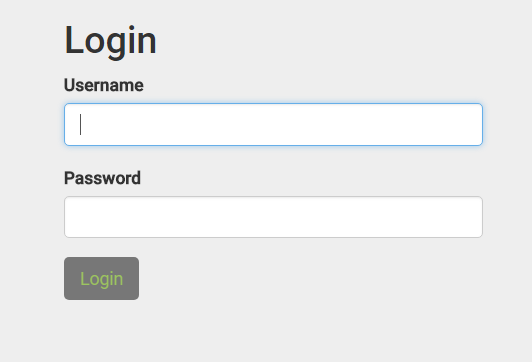
\includegraphics[width=\textwidth]{AS/login/1}
\end{center}
\caption{Login Page}
\end{figure}

\item If you have forgotten the password to your account, then please click on 'Reset Password' option in the login menu. Fill the form with the email connected to your account. If everything has gone well, the information about a sent email will be displayed.

\begin{figure}[h!]
\begin{center}
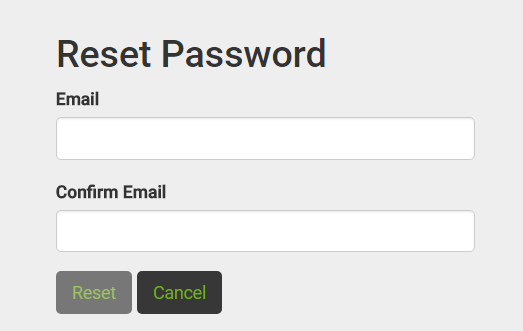
\includegraphics[width=\textwidth]{AS/login/4}
\end{center}
\caption{Reset Password Page}
\end{figure}

\item If you manage to successfully log in, welcome message and side menu on the left side of the page will appear.
\begin{figure}[h!]
\begin{center}
\includegraphics[width=\textwidth]{AS/login/2}
\end{center}
\caption{Welcome Page shown after logging in}
\end{figure}

\item Depending on role assigned to your account, different subpages will be available. For instance, only manager can edit user accounts.

\begin{figure}[h!]
\begin{center}
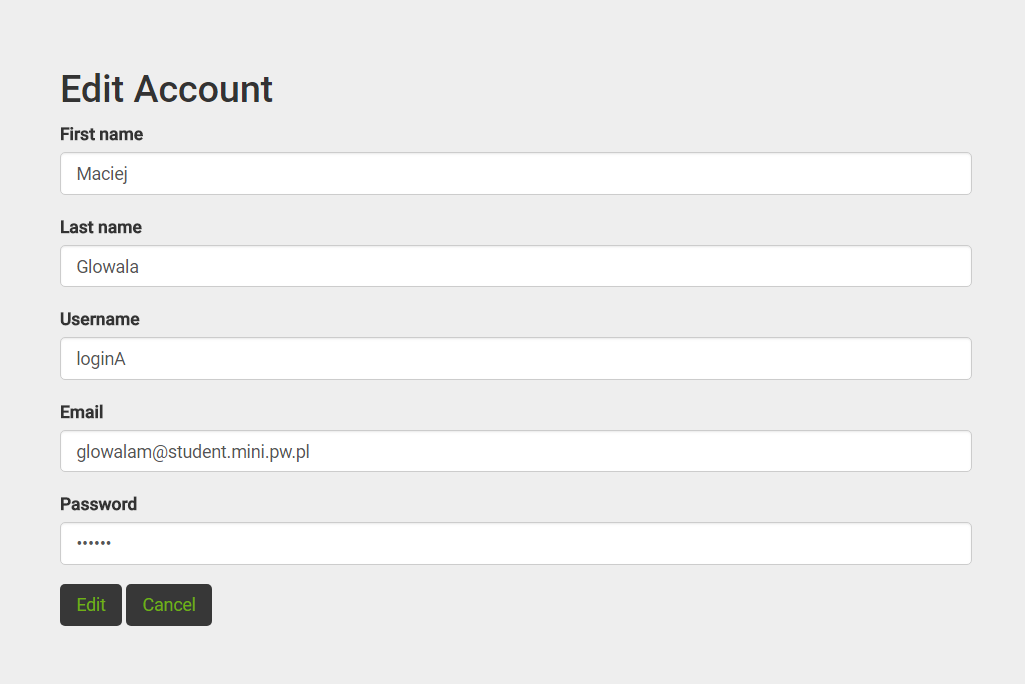
\includegraphics[width=\textwidth]{AS/login/5}
\end{center}
\caption{Edit User Account Page}
\end{figure}

\item You can log out using ‘Log Out’ button
\begin{figure}[h!]
\begin{center}
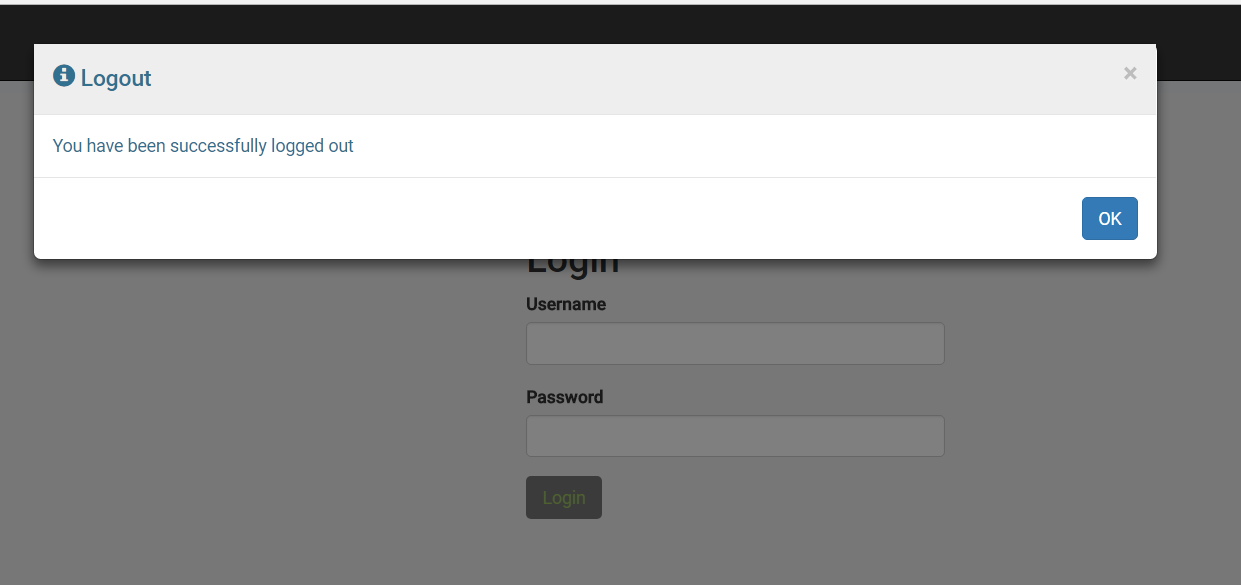
\includegraphics[width=\textwidth]{AS/login/3}
\end{center}
\caption{Page seen after logging out}
\end{figure}
\end{enumerate}
\section{Resources}
\begin{enumerate}
\item To manage resources, please click on 'Resources' in the left side menu. 
\begin{figure}[h!]
\begin{center}
\includegraphics[width=\textwidth]{AS/resources/1}
\end{center}
\caption{Manage Resources Page}
\end{figure}
\thispagestyle{empty}
\item In order to add a new resource, click ‘Add New Resource’, then fill in the form. In the ‘Image’ field, please provide an image from your computer library and click 'Save'.

\begin{figure}[h!]
\begin{center}
\includegraphics[width=\textwidth]{AS/resources/2}
\end{center}
\caption{Add Resource}
\end{figure}
\thispagestyle{empty}

\item In order to view resource details, please click on the magnifying glass next to it.

\begin{figure}[h!]
\begin{center}
\includegraphics[width=\textwidth]{AS/resources/3}
\end{center}
\caption{View Resource}
\end{figure}
\thispagestyle{empty}

\item To edit a resource, please click on the pencil icon next to it. Enter the changes and click ‘Update’. If you will leave image input empty, the old photo will be inserted and the image will not be changed.

\begin{figure}[h!]
\begin{center}
\includegraphics[width=\textwidth]{AS/resources/4}
\end{center}
\caption{Edit Resource}
\end{figure}
\thispagestyle{empty}

\item To delete a resource, please click on the bin icon next to it and then confirm.
\end{enumerate}


\begin{figure}[h!]
\begin{center}
\includegraphics[width=\textwidth]{AS/resources/5}
\end{center}
\caption{Delete Resource}
\end{figure}
\thispagestyle{empty}

\section{Products}
\begin{enumerate}
\item To manage products, please click on 'Products' in the left side menu. 
\begin{figure}[h!]
\begin{center}
\includegraphics[width=\textwidth]{AS/product/1}
\end{center}
\caption{Manage Products Page}
\end{figure}
\thispagestyle{empty}

\item To add a new product, please click ‘Add New Product’, then fill in the form. In the ‘Image’ field, please provide an image from your computer library and click 'Save'.
\begin{figure}[h!]
\begin{center}
\includegraphics[width=\textwidth]{AS/product/4}
\end{center}
\caption{Add Product}
\end{figure}
\thispagestyle{empty}

\item In order to view product details, please click on the magnifying glass next to it.

\begin{figure}[h!]
\begin{center}
\includegraphics[width=\textwidth]{AS/product/5}
\end{center}
\caption{View Product}
\end{figure}
\thispagestyle{empty}


\item To edit a product, please click on the pencil icon next to it. Enter the changes and click ‘Update’. If you will leave the image input empty, the old photo will be inserted and the image will not be changed.

\begin{figure}[h!]
\begin{center}
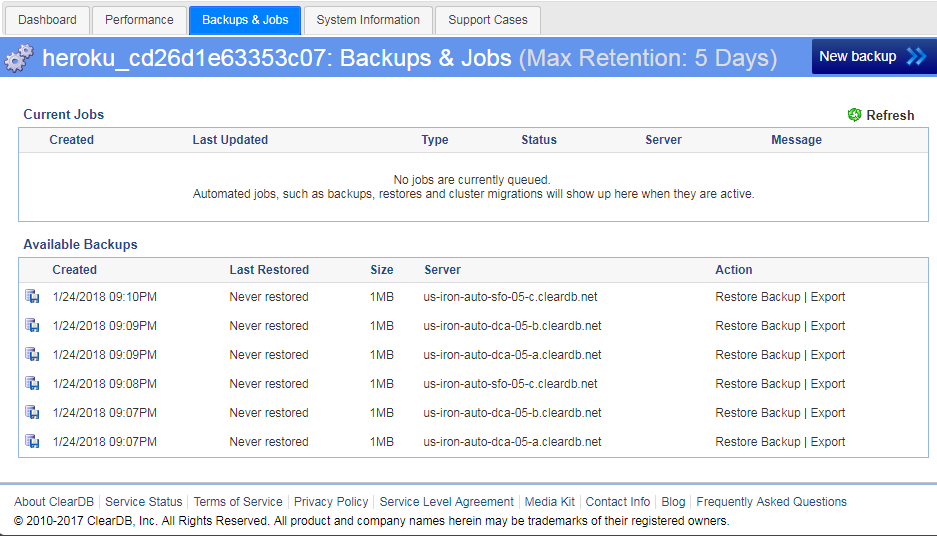
\includegraphics[width=\textwidth]{AS/product/6}
\end{center}
\caption{Edit Product}
\end{figure}
\thispagestyle{empty}

\item To delete a product, please click the bin icon next to it and then confirm.


\begin{figure}[h!]
\begin{center}
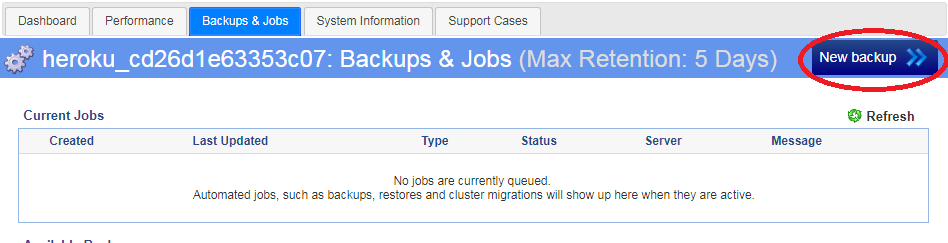
\includegraphics[width=\textwidth]{AS/product/7}
\end{center}
\caption{Delete Product}
\end{figure}
\thispagestyle{empty}

\item To view a formula for the chosen product, please click on the magnifying glass in the formula column.

\begin{figure}[h!]
\begin{center}
\includegraphics[width=\textwidth]{AS/product/2}
\end{center}
\caption{View of a product's formula}
\end{figure}
\thispagestyle{empty}

\item To edit a formula of the chosen product, please click the on the pencil in the formula column. Check the resources you want to add to formula and fill the quantity of each in the input box next to resource name. If you are done, please click ‘Save’.


\begin{figure}[h!]
\begin{center}
\includegraphics[width=\textwidth]{AS/product/3}
\end{center}
\caption{Edit product's formula Page}
\end{figure}
\thispagestyle{empty}
\end{enumerate}

\section{Orders}
\begin{enumerate}
\item To send an order to the resource suppliers, please check resources you wish to order and fill their quantity in the input box next to resource name.
Then please click ‘Send Order’.

\begin{figure}[h!]
\begin{center}
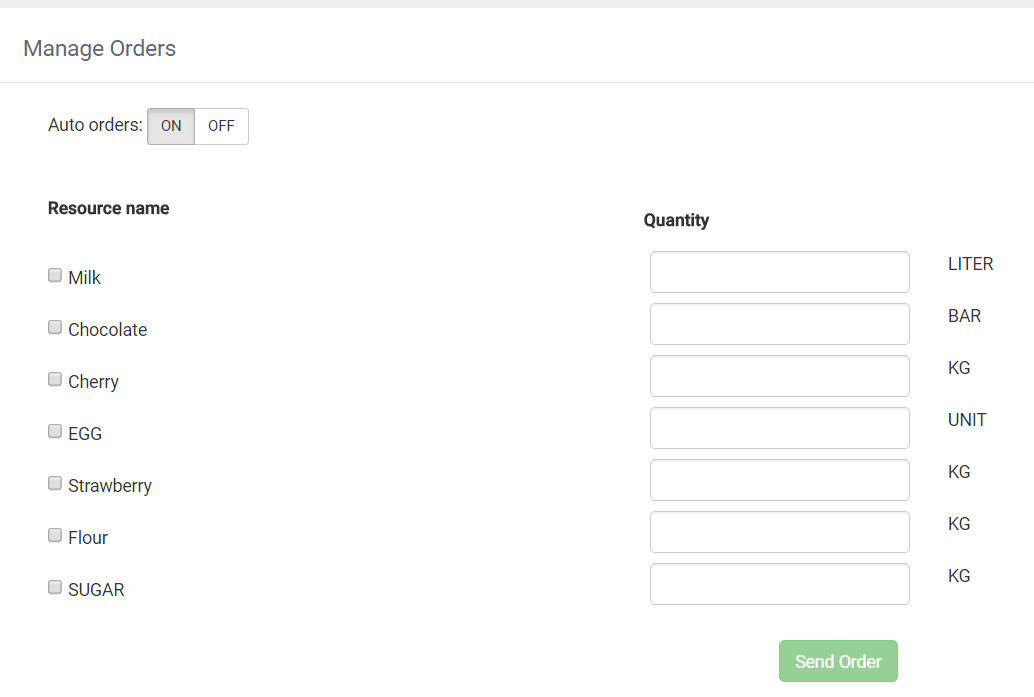
\includegraphics[width=\textwidth]{AS/orders/1}
\end{center}
\caption{Manage Orders Page}
\end{figure}
\thispagestyle{empty}

\end{enumerate}

\section{Report generation for resource and product}
\begin{enumerate}
\item To generate a report please check resources/products for which you would like to see the report. Then please choose a chart type, the last date that will be in the scope of the report and for how many days back should the report be generated. If you just want to display report in the browser - click ‘Generate Report’. If you want to receive report via email, please fill also ‘email of receiver’ input box and click ‘Send report’.

\begin{figure}[h!]
\begin{center}
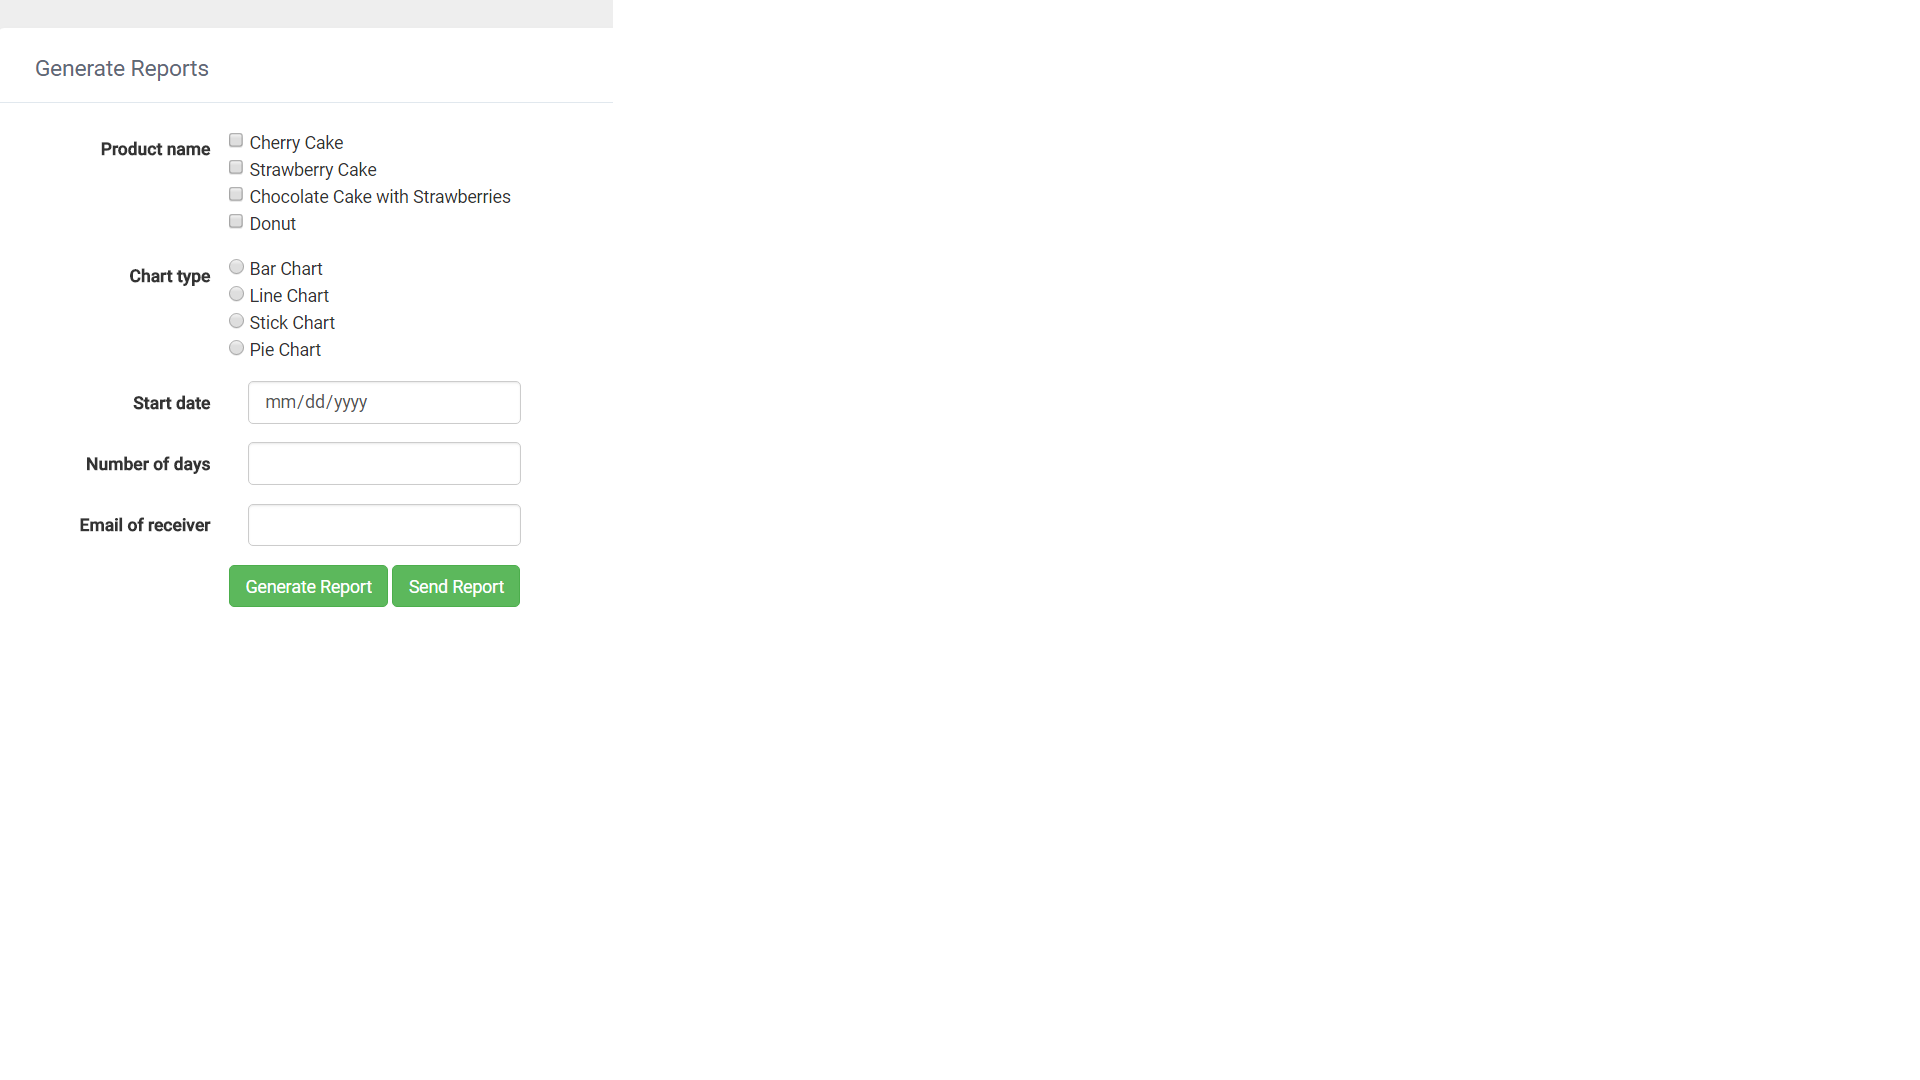
\includegraphics[scale = 1]{AS/report/1}
\end{center}
\caption{Generate and Send Product Report}
\end{figure}
\thispagestyle{empty}

\begin{figure}[h!]
\begin{center}
\includegraphics[scale = 1]{AS/report/3}
\end{center}
\caption{Generate and Send Resource Usage Report}
\end{figure}
\thispagestyle{empty}


\end{enumerate}

\section{Forecast Report for Resource and Product}
\begin{enumerate}
\item To generate forecast report please check resources/products for which you would like to see the report, choose chart type, the last date that will be in the scope of the report, how many days back should the report go and for how many days you would like to generate forecast report. If you want to just display report in the browser – please click on "Generate Forecast". If you want to receive report via email, please fill also "Email of receiver" input box and click "Send Forecast".

\begin{figure}[h!]
\begin{center}
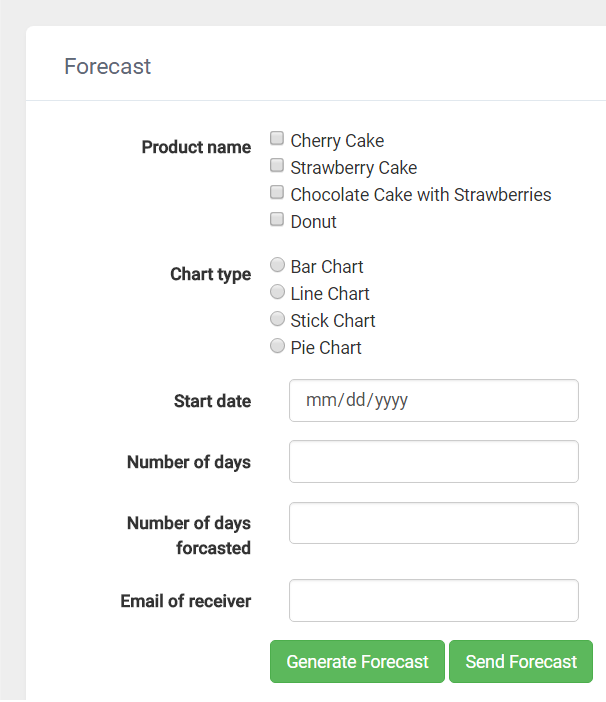
\includegraphics[scale = 1]{AS/report/2}
\end{center}
\caption{Generate and Send Production Forecast Report}
\end{figure}
\thispagestyle{empty}

\begin{figure}[h!]
\begin{center}
\includegraphics[scale = 1]{AS/report/4}
\end{center}
\caption{Generate and Send Resource Usage Forecast Report}
\end{figure}
\thispagestyle{empty}


\end{enumerate}
\section{Categories of products and resources}
\begin{enumerate}
\item To manage categories of products and resources, please click on 'Manage Categories' in the left side menu, and choose ‘Products’ or ‘Resources’ subpage.
\begin{figure}[h!]
\begin{center}
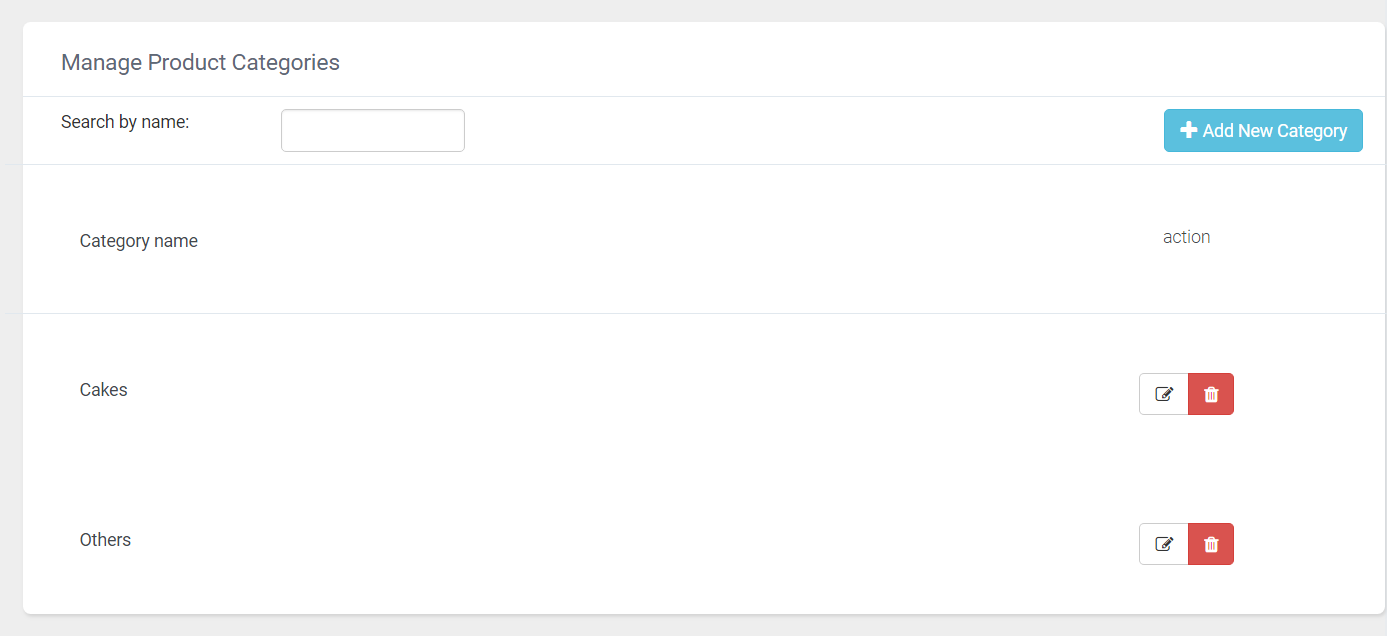
\includegraphics[width=\textwidth]{AS/categories/product/1}
\end{center}
\caption{Manage Product Categories View}
\end{figure}

\begin{figure}[h!]
\begin{center}
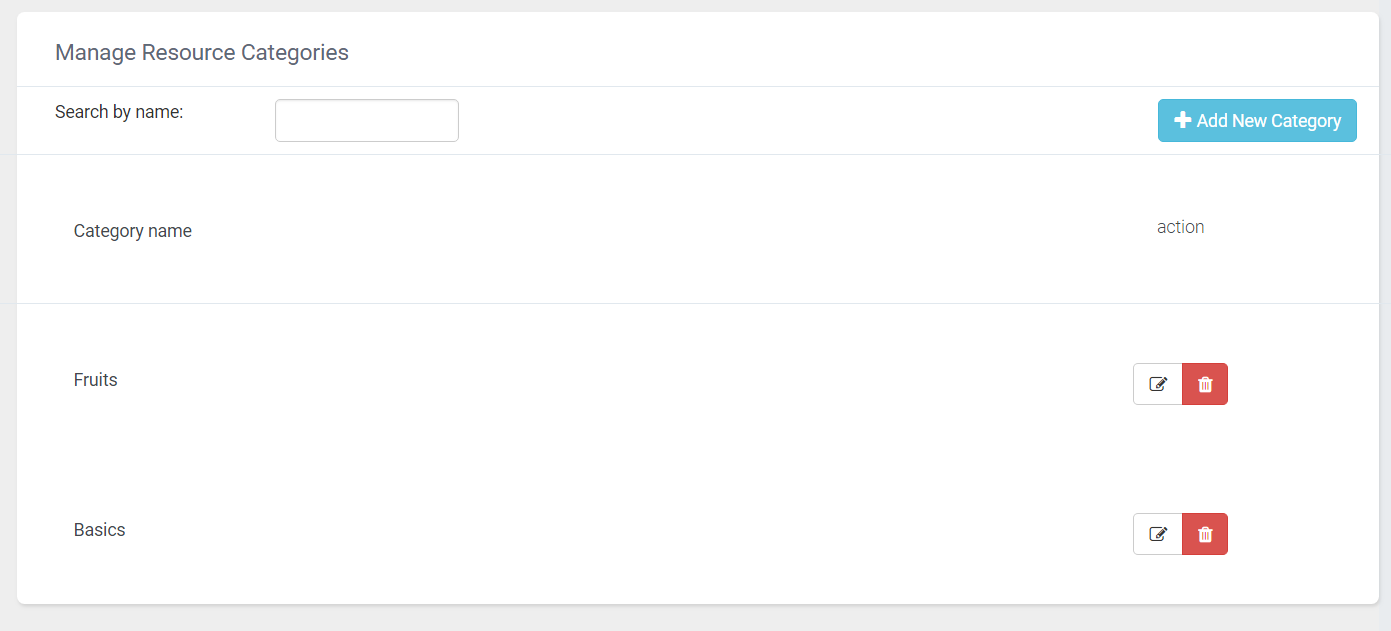
\includegraphics[width=\textwidth]{AS/categories/resource/1}
\end{center}
\caption{Manage Resource Categories View}
\end{figure}

\item To add new category, click ‘Add New Category’. Than please fill in the form with category name and click 'Save'.
\begin{figure}[h!]
\begin{center}
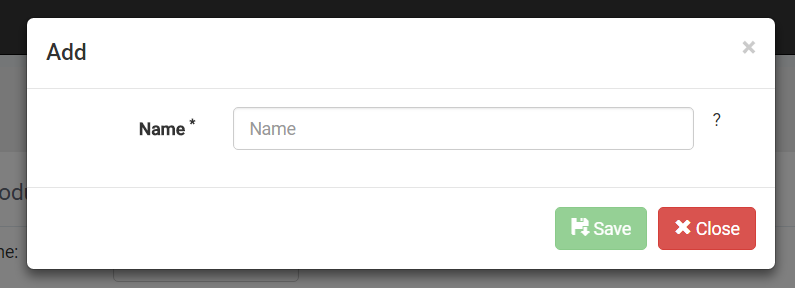
\includegraphics[width=\textwidth]{AS/categories/product/2}
\end{center}
\caption{Add Product Category}
\end{figure}


\begin{figure}[h!]
\begin{center}
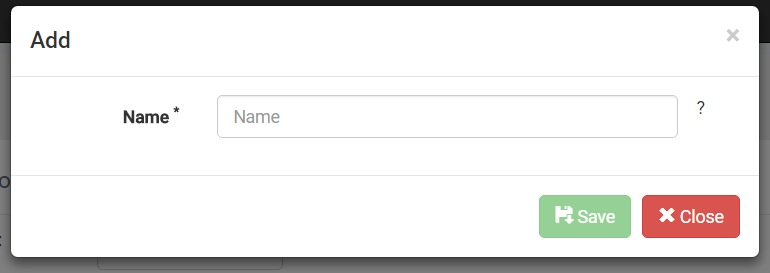
\includegraphics[width=\textwidth]{AS/categories/resource/2}
\end{center}
\caption{Add Resource Category}
\end{figure}

\item To edit category, please click on the pencil icon next to it. Enter the changes and click ‘Update’ to save. 


\begin{figure}[h!]
\begin{center}
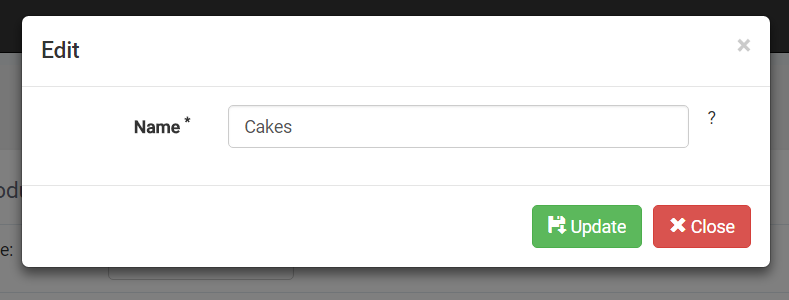
\includegraphics[width=\textwidth]{AS/categories/product/3}
\end{center}
\caption{Edit Product Category}
\end{figure}

\begin{figure}[h!]
\begin{center}
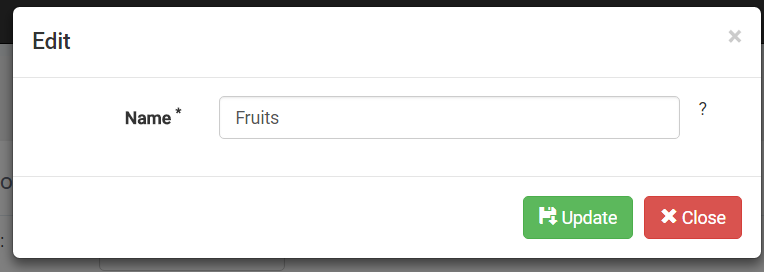
\includegraphics[width=\textwidth]{AS/categories/resource/3}
\end{center}
\caption{Edit Resource Category}
\end{figure}

\item To delete category, please click the bin icon next to it and then confirm. You will not be able to delete category, if any products/resources are in this category – you will need to reassign these products/resources to a different category and then try to delete the category.

\begin{figure}[h!]
\begin{center}
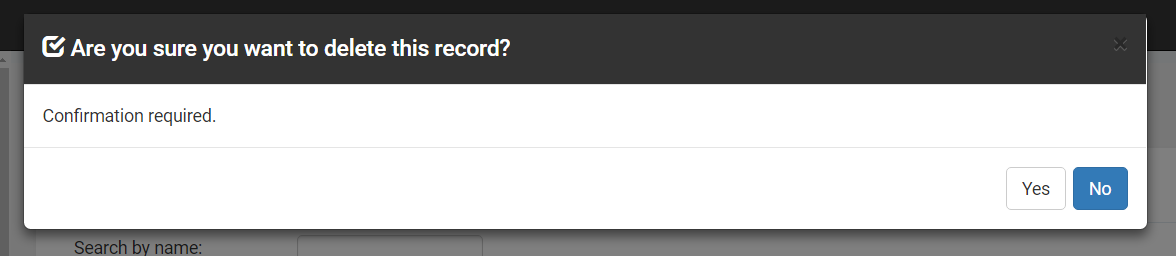
\includegraphics[width=\textwidth]{AS/categories/product/4}
\end{center}
\caption{Delete Product Category}
\end{figure}

\begin{figure}[h!]
\begin{center}
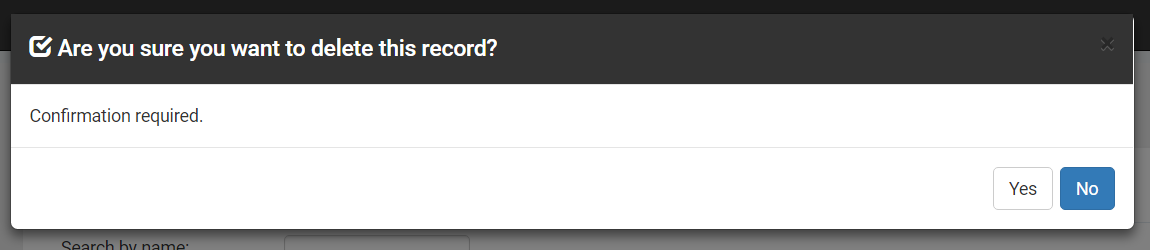
\includegraphics[width=\textwidth]{AS/categories/resource/4}
\end{center}
\caption{Delete}
\end{figure}

\end{enumerate}

\section{Notifications}
\begin{enumerate}

\item To manage notifications, please click on ‘Notifications’ in the left side menu. 


\begin{figure}[h!]
\begin{center}
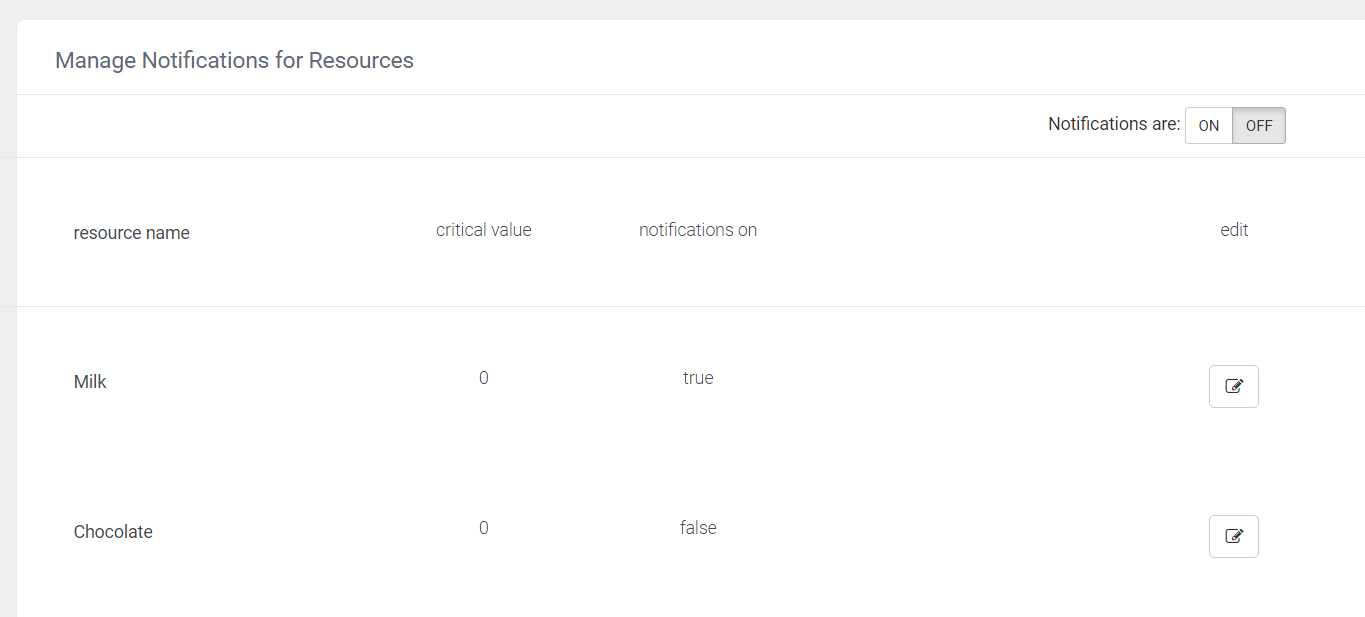
\includegraphics[width=\textwidth]{AS/notifications/1}
\end{center}
\caption{Manage Notifications Page}
\end{figure}


\item To a edit notification for chosen resource, please click on the pencil icon next to it. Enter critical value – an amount of a resource low enough to trigger the notifications and turn notifications on or off.

\begin{figure}[h!]
\begin{center}
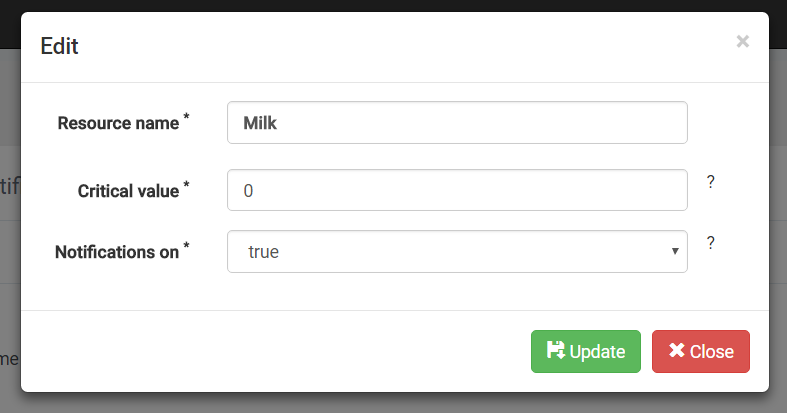
\includegraphics[width=\textwidth]{AS/notifications/2}
\end{center}
\caption{Edit a notification}
\end{figure}
\thispagestyle{empty}

\item You can also turn on/off notifications for all available resources by clicking on ‘Notifications are’ switch on the top of the page
\end{enumerate}

\section{Suppliers}
\begin{enumerate}
\item To manage suppliers, please click on ‘Suppliers’ in the left side menu. 

\begin{figure}[h!]
\begin{center}
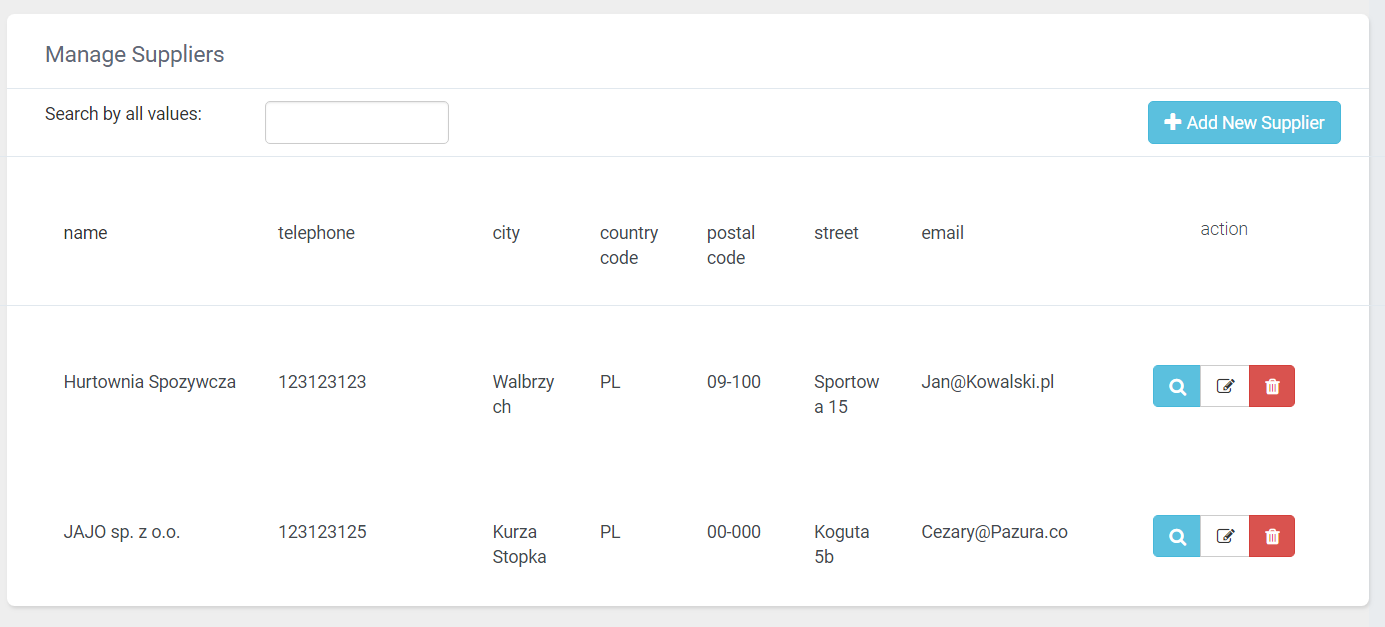
\includegraphics[width=\textwidth]{AS/supplier/1}
\end{center}
\caption{Manage Suppliers View}
\end{figure}
\thispagestyle{empty}

\item To add new supplier, click ‘Add New Supplier. Than fill in the form and click 'save'.

\begin{figure}[h!]
\begin{center}
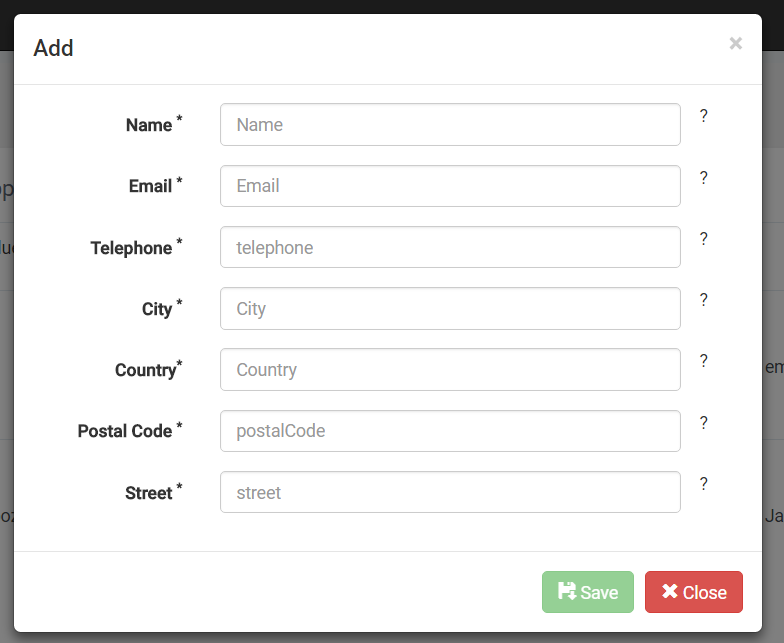
\includegraphics[width=\textwidth]{AS/supplier/2}
\end{center}
\caption{Add Supplier}
\end{figure}
\thispagestyle{empty}
\item To view chosen supplier details, please click the magnifying glass next to it.

\begin{figure}[h!]
\begin{center}
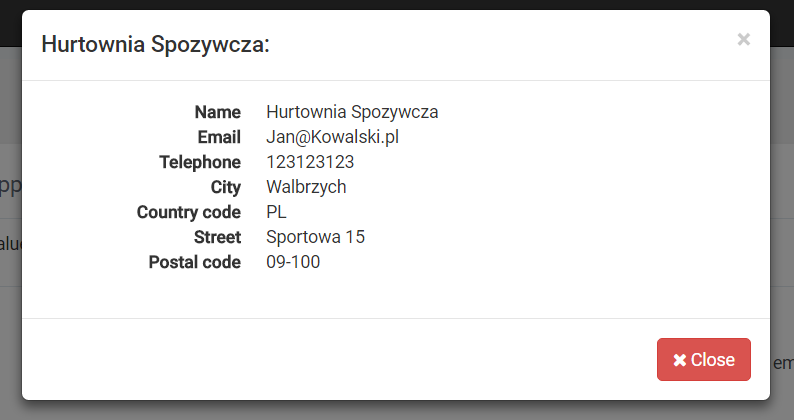
\includegraphics[width=\textwidth]{AS/supplier/3}
\end{center}
\caption{View Supplier}
\end{figure}
\thispagestyle{empty}

\item To edit supplier’s details, please click on the pencil icon next to it. Enter the changes and click update. 

\begin{figure}[h!]
\begin{center}
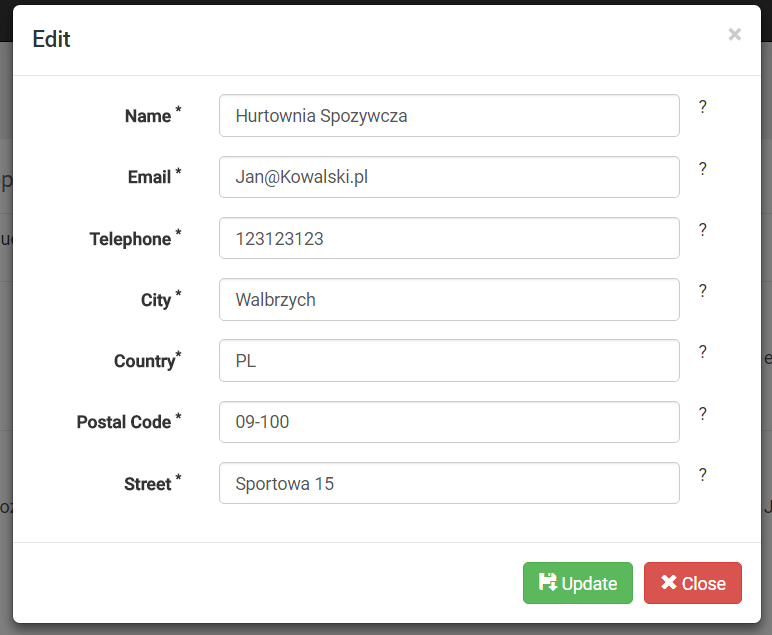
\includegraphics[width=\textwidth]{AS/supplier/4}
\end{center}
\caption{Edit Supplier}
\end{figure}
\thispagestyle{empty}
\item To delete a supplier, please click the bin icon next to it and then confirm.

\begin{figure}[h!]
\begin{center}
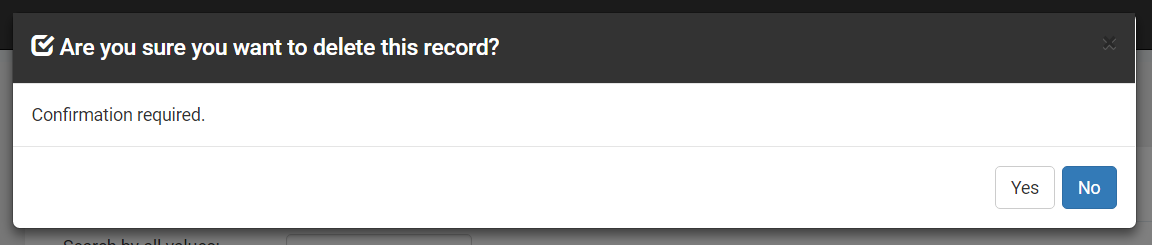
\includegraphics[width=\textwidth]{AS/supplier/5}
\end{center}
\caption{Delete Supplier}
\end{figure}

\end{enumerate}



\section{Jobs}
\begin{enumerate}
\item To manage jobs, please click on ‘Manage Jobs’ in the left side menu. 

\begin{figure}[h!]
\begin{center}
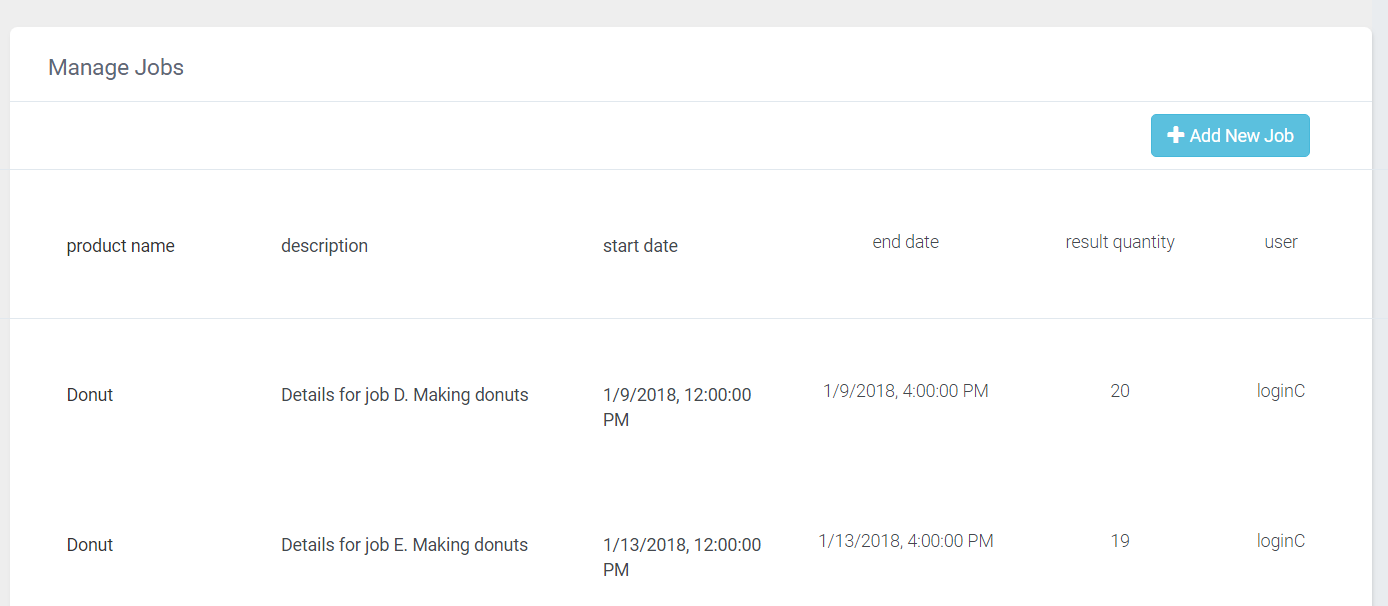
\includegraphics[width=\textwidth]{AS/jobs/1}
\end{center}
\caption{Manage Jobs View}
\end{figure}



\item To add new job, please click on ‘Add New Job’. Then fill in the form and click 'Save'. Username which is displayed in the table next to each job will be added automatically, It will be a login of the user adding the job.
\begin{figure}[h!]
\begin{center}
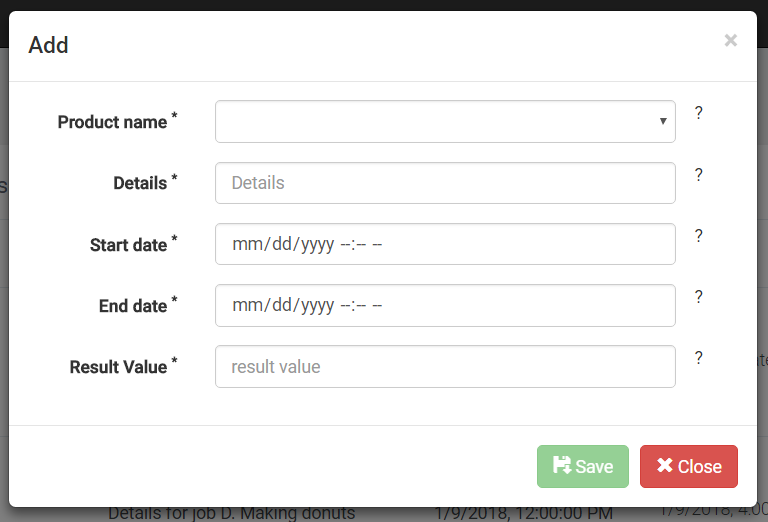
\includegraphics[width=\textwidth]{AS/jobs/2}
\end{center}
\caption{Add New Job}
\end{figure}
\thispagestyle{empty}


\end{enumerate} 
\section{Users}
\begin{enumerate}
\item To manage users, please click on ‘Manage Users’ in the left side menu. 


\begin{figure}[h!]
\begin{center}
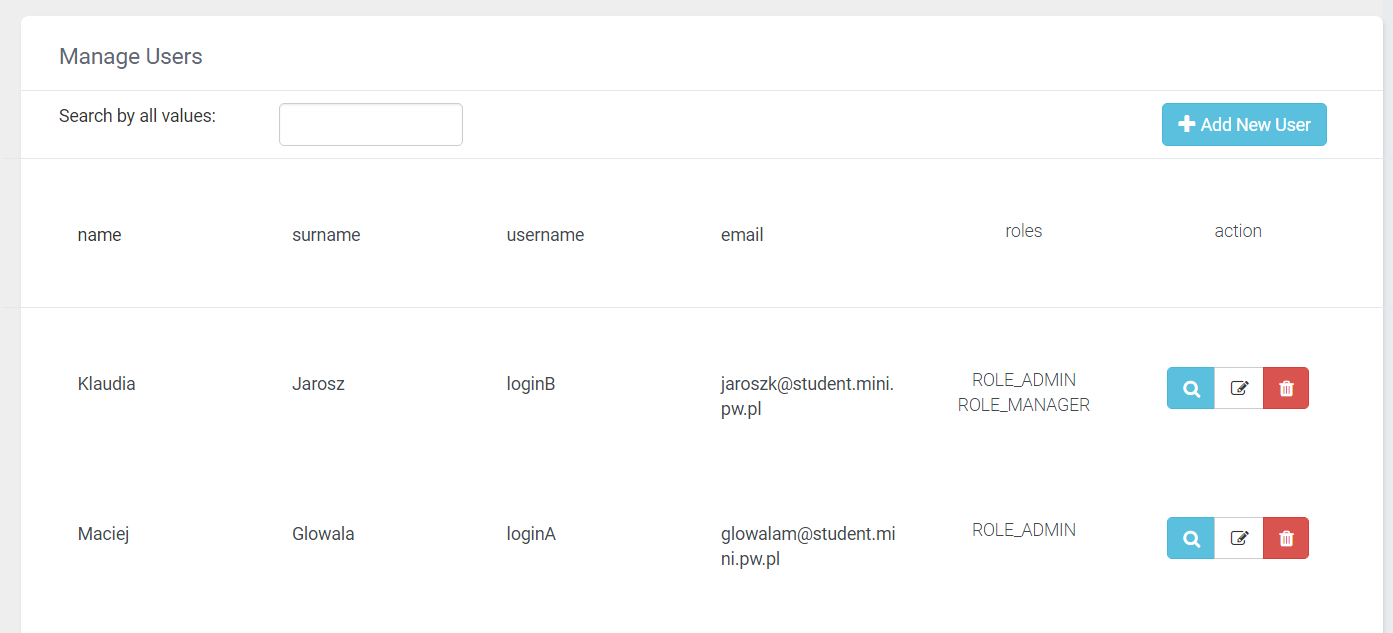
\includegraphics[width=\textwidth]{AS/users/1}
\end{center}
\caption{Manage Users Page}
\end{figure}
\thispagestyle{empty}


\item To add new user, please click on ‘Add New User’. Then fill in the form and click 'Save'. Note: Be careful when choosing the role for the user - administrator role gives user access to sensitive data.

\begin{figure}[h!]
\begin{center}
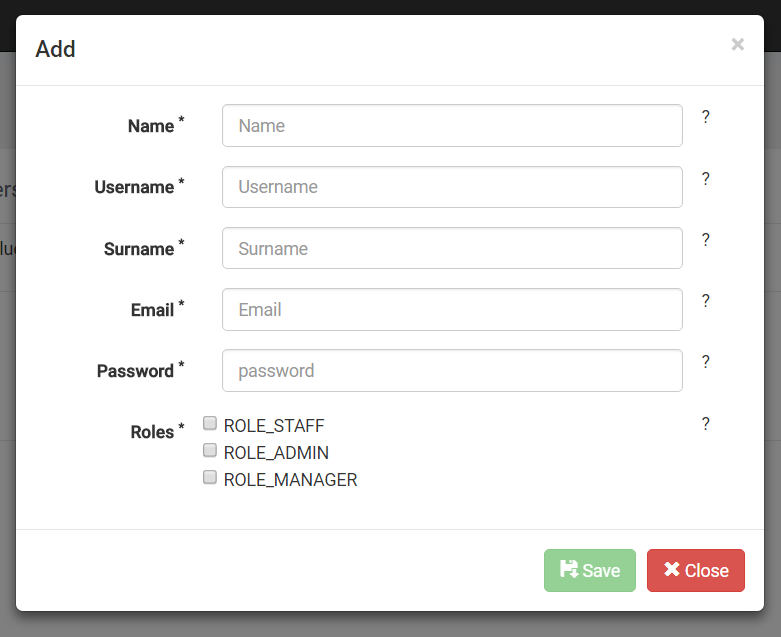
\includegraphics[width=\textwidth]{AS/users/2}
\end{center}
\caption{Add User}
\end{figure}
\thispagestyle{empty}


\item To view details for a chosen user, please click on the magnifying glass next to it.


\begin{figure}[h!]
\begin{center}
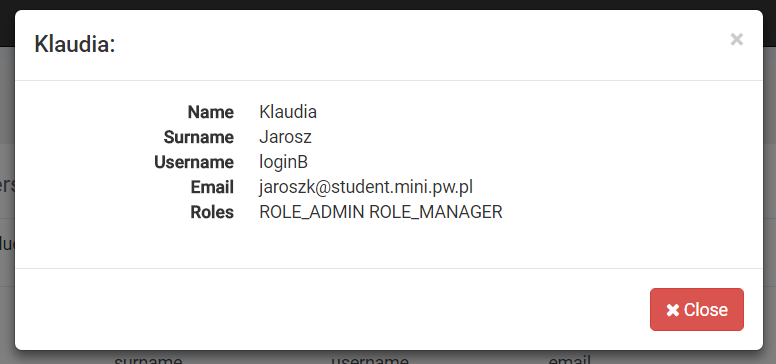
\includegraphics[width=\textwidth]{AS/users/3}
\end{center}
\caption{View User}
\end{figure}
\thispagestyle{empty}
\item To edit user details, please click on the pencil icon next to it. Enter the changes and click update. 


\begin{figure}[h!]
\begin{center}
\includegraphics[width=\textwidth]{AS/users/4}
\end{center}
\caption{Edit User}
\end{figure}
\thispagestyle{empty}

\item To delete user, please click on the bin icon next to it and then confirm.


\begin{figure}[h!]
\begin{center}
\includegraphics[width=\textwidth]{AS/users/5}
\end{center}
\caption{Delete User}
\end{figure}
\thispagestyle{empty}


\end{enumerate}

\section{Database Recovery}

There is database dump nightly scheduled on the hosted server. There are up to 5 days backups stored. You can also perform a backup manually any time.
\subsection{Management}
\begin{enumerate}
\item Please go to hosting server: https://id.heroku.com/login and log in.
\item Please Choose mini-lime from application list.
\item Then, click on ClearDB MySQL in the overview tab.
\item Please Select DataBase.
\item Then, please select Backups \& Jobs tab.
 \end{enumerate}

\begin{figure}[h!]
\begin{center}
\includegraphics[scale = 1]{DB/1}
\end{center}
\caption{DataBase Management}
\end{figure}
\thispagestyle{empty}
\begin{figure}[h!]
\begin{center}
\includegraphics[scale = 1]{DB/2}
\end{center}
\caption{DataBase Management}
\end{figure}
\thispagestyle{empty}
\begin{figure}[h!]
\begin{center}
\includegraphics[scale = 1]{DB/3}
\end{center}
\caption{DataBase Management}
\end{figure}
\thispagestyle{empty}
\begin{figure}[h!]
\begin{center}
\includegraphics[width=\textwidth]{DB/4}
\end{center}
\caption{DataBase Management}
\end{figure}
\thispagestyle{empty}
\begin{figure}[h!]
\begin{center}
\includegraphics[width=\textwidth]{DB/5}
\end{center}
\caption{DataBase Management}
\end{figure}
\thispagestyle{empty}
\begin{figure}[h!]
\begin{center}
\includegraphics[width=\textwidth]{DB/6}
\end{center}
\caption{DataBase Management}
\end{figure}
\thispagestyle{empty}


\subsection{DataBase dump} 
\begin{enumerate}
\item Please click 'New Backup'.
\item Please wait until queued job is done.
\end{enumerate}


\begin{figure}[h!]
\begin{center}
\includegraphics[width=\textwidth]{DB/7}
\end{center}
\caption{DataBase dump}
\end{figure}
\thispagestyle{empty}
\begin{figure}[h!]
\begin{center}
\includegraphics[width=\textwidth]{DB/8}
\end{center}
\caption{DataBase dump}
\end{figure}
\thispagestyle{empty}

\subsection{Restore DataBase} 
\begin{enumerate}
\item Please choose BackUp from a list and then click 'Restore Backup' and confirm.
\item Please wait until queued job is done.
\end{enumerate}
\begin{figure}[h!]
\begin{center}
\includegraphics[width=\textwidth]{DB/9}
\end{center}
\caption{Restore DataBase}
\end{figure}
\thispagestyle{empty}
\begin{figure}[h!]
\begin{center}
\includegraphics[scale = 1]{DB/10}
\end{center}
\caption{Restore DataBase}
\end{figure}
\thispagestyle{empty}

\begin{figure}[h!]
\begin{center}
\includegraphics[width=\textwidth]{DB/11}
\end{center}
\caption{Restore DataBase}
\end{figure}
\thispagestyle{empty}














% -----------------------------  APPENDIX B ---------------------------
\chapter{Appendix B: Test Report}

\subsection{Unit Tests} The application was throughly tested. The team performed almost a hundred of Unit Tests. The detailed report can be found and browsed in "Unit Test Reports" catalog by launching the file index.html.
\subsection{Scenario Tests} Hence presented is a summary of scenario tests performed:

\begin{longtable}{|p{1cm}|p{11cm}|p{4cm}|}
\caption[Scenario Test Summary]{Scenario Test Summary}
\label{Scenario Test Summary}
\centering
\tabularnewline

\hline
\textbf{\#} & \textbf{Scenario} & \textbf{Test Result} \\ \hline
1 & An administrator logs in to the system & Passed \\ \hline
2 & An administrator changes his password & Passed \\ \hline
3 & An administrator creates a user account in the system. Then he checks in the Users view if the account has appeared & Passed \\ \hline
4 & An administrator modifies a user account in the system. Then he checks in the Users view if the account has been changed & Passed \\ \hline
5 & An administrator deletes a user account in the system. Then he checks in the Users view if the account has disappeared & Passed \\ \hline
6 & An administrator creates a resource in the system. Then he checks in the Resources view if the resource has appeared and if it looks properly & Passed \\ \hline
7 & An administrator modifies a resource in the system. Then he checks in the Resources view if the resource has changed its details & Passed \\ \hline
8 & An administrator deletes a resource in the system. Then he checks in the Resources view if the resource has disappeared & Passed \\ \hline
9 & An administrator creates a product in the system. Then he checks in the Products view if the product has appeared and if it looks properly & Passed \\ \hline
10 & An administrator modifies a product in the system. Then he checks in the Products view if the product has changed its details & Passed \\ \hline
11 & An administrator deletes a product in the system. Then he checks in the Products view if the product has disappeared & Passed \\ \hline

12 & An administrator creates a category of resources in the system and assigns some resources to it. Then he checks in the Category -> Resources view if the category has appeared and if has proper resources assigned to it & Passed \\ \hline
13 & An administrator modifies a category of resources in the system and assigns different resources to it. Then he checks in the Category -> Resources view if the category has proper resources assigned to it & Passed \\ \hline
14 & An administrator deletes a (previously emptied) category of resources in the system. Then he checks in the Category -> Resources view if the category has disappeared & Passed \\ \hline
15 & An administrator creates a category of products in the system and assigns some products to it. Then he checks in the Category -> Products view if the category has appeared and if has proper products assigned to it & Passed \\ \hline
16 & An administrator modifies a category of products in the system and assigns different products to it. Then he checks in the Category -> Products view if the category has proper products assigned to it & Passed \\ \hline
17 & An administrator deletes a (previously emptied) category of products in the system. Then he checks in the Category -> Products view if the category has disappeared & Passed \\ \hline


18 & An administrator creates a formula for a product in the system and assigns some resources to it. Then he checks in the Products view if the formula has appeared with proper resources assigned to it & Passed \\ \hline
19 & An administrator modifies a formula for a product in the system and assigns different resources to it. Then he checks in the Products view if the formula has proper resources assigned to it & Passed \\ \hline

20 & An administrator creates a report for some a product in the system and chooses some time period. He inputs his own email address and clicks 'Send report'. Then he checks in the inbox if he had received a report and if the looks of it appear properly & Passed \\ \hline
21 & An administrator creates a report for some a resource in the system and chooses some time period. He inputs his own email address and clicks 'Send report'. Then he checks in the inbox if he had received a report and if the looks of it appear properly & Passed \\ \hline
22 & An administrator creates a forecast report for some a product in the system and chooses some time period. He inputs his own email address and clicks 'Send report'. Then he checks in the inbox if he had received a report and if the looks of it appear properly & Passed \\ \hline
23 & An administrator creates a forecast report for some a resource in the system and chooses some time period. He inputs his own email address and clicks 'Send report'. Then he checks in the inbox if he had received a report and if the looks of it appear properly & Passed \\ \hline

24 & An administrator creates a supplier in the system. Then he checks in the Suppliers view if the supplier has appeared and if it looks properly & Passed \\ \hline
25 & An administrator modifies a supplier in the system. Then he checks in the Suppliers view if the supplier has changed its details & Passed \\ \hline
26 & An administrator deletes a supplier in the system. Then he checks in the Suppliers view if the supplier has disappeared & Passed \\ \hline

27 & An administrator creates a job and declare time range. Then he checks in the Jobs view if the job has appeared and if it looks properly and includes his own username & Passed \\ \hline
28 & An administrator defines a notifications, turns notifications on. He performs a job where he reduces the amount of resource to a critical value. Then he checks in the inbox if he had received a notification about a low level of resource and if the looks of it appear properly & Passed \\ \hline
29 & An administrator defines a notifications, turns notifications off. He performs a job where he reduces the amount of resource to a critical value. Then he checks in the inbox if he had recived nothing as expected & Passed \\ \hline

30 & An administrator substitutes one of the supplier email addresses with his own. Then he orders the resources and checks in the inbox if he had received an order & Passed \\ \hline

31 & An administrator substitutes one of the supplier email addresses with his own. He turns on automatic ordering. He performs a job where he reduces the amount of resource to a critical value. Then he checks in the inbox if he had received an order & Passed \\ \hline


\end{longtable}

\thispagestyle{empty}


\end{document}
